\chapter{LZ Sensitivity Studies}
\label{chap:chap5}

Understanding the physical response of a detector to its environment is key in assessing the capacity of the detector in looking for the desired physics objectives. Furthermore, detector design has to take into account this response to optimise construction and allow for the testing of theories and models by comparison to data. Over the past few years, the LZ simulation and statistical packages were developed alongside the design and construction of the experiment. The focus of this chapter is initially to give a brief introduction to these packages, focusing primarily on the statistical software package \textsc{LZStats}, which has been developed and used to study the sensitivity and discovery potential of the experiment to WIMP dark matter. Moreover, as part of this study, the impact of radon for the WIMP search is examined.


%%------------------------------$$
\section{Overview}
\label{sec:overview_5}
%%------------------------------$$

The instruments used in pursuit of new physics becomes a playground in which new discoveries can be made. However, without fully understanding the internal dynamics of this playground and the precise response mechanics taking place as a result of known (background) and unknown (signal) interactions, the ability to claim a discovery is diminished. Simulation of detectors through the means of Monte Carlo modeling is an essential tool in physics to test theories and models by comparison to data, and more importantly, to understand the response dynamics of such a playground to these interactions. 

Although the origin of background events and their response mechanisms in LXe are well understood, this alone is not enough to determine the actual rates observed by the entire system operating in unison. The simulation of events for LZ serves multiple purposes; the primary of which is to determine an optimal detector design that takes into account material specific background rates, and their physical and geometric features in constructing an ultra low-background detector optimised for the detection of WIMPs. Furthermore, upon a verified detector design, the simulations are used for the calculation of background rates in LZ with input from radioactivity measurements. Through the use of these rates and by utilising on a Profile Likelihood Ratio analysis (PLR), the sensitivity of the experiment to various rare event searches is predicted. 

The LZ simulation chain brings together a class of packages that simulate the response of the detector beginning from the initial interaction point---the point of first energy deposition, all the way through the electronic and algorithmic response models in creating an ultra-realistic event topology. The chain beings with a \textsc{Geant4} based in-house code \textsc{BACCARAT} to track the passage of particles through the detector, identifying and recording their interaction points. The output from \textsc{BACCARAT} is further used in two separate chains as detailed in figure (\ref{fig:lz_simulation_chains}). 

%
\begin{figure}[b]
    \centering
    \hspace*{-0.2cm}
    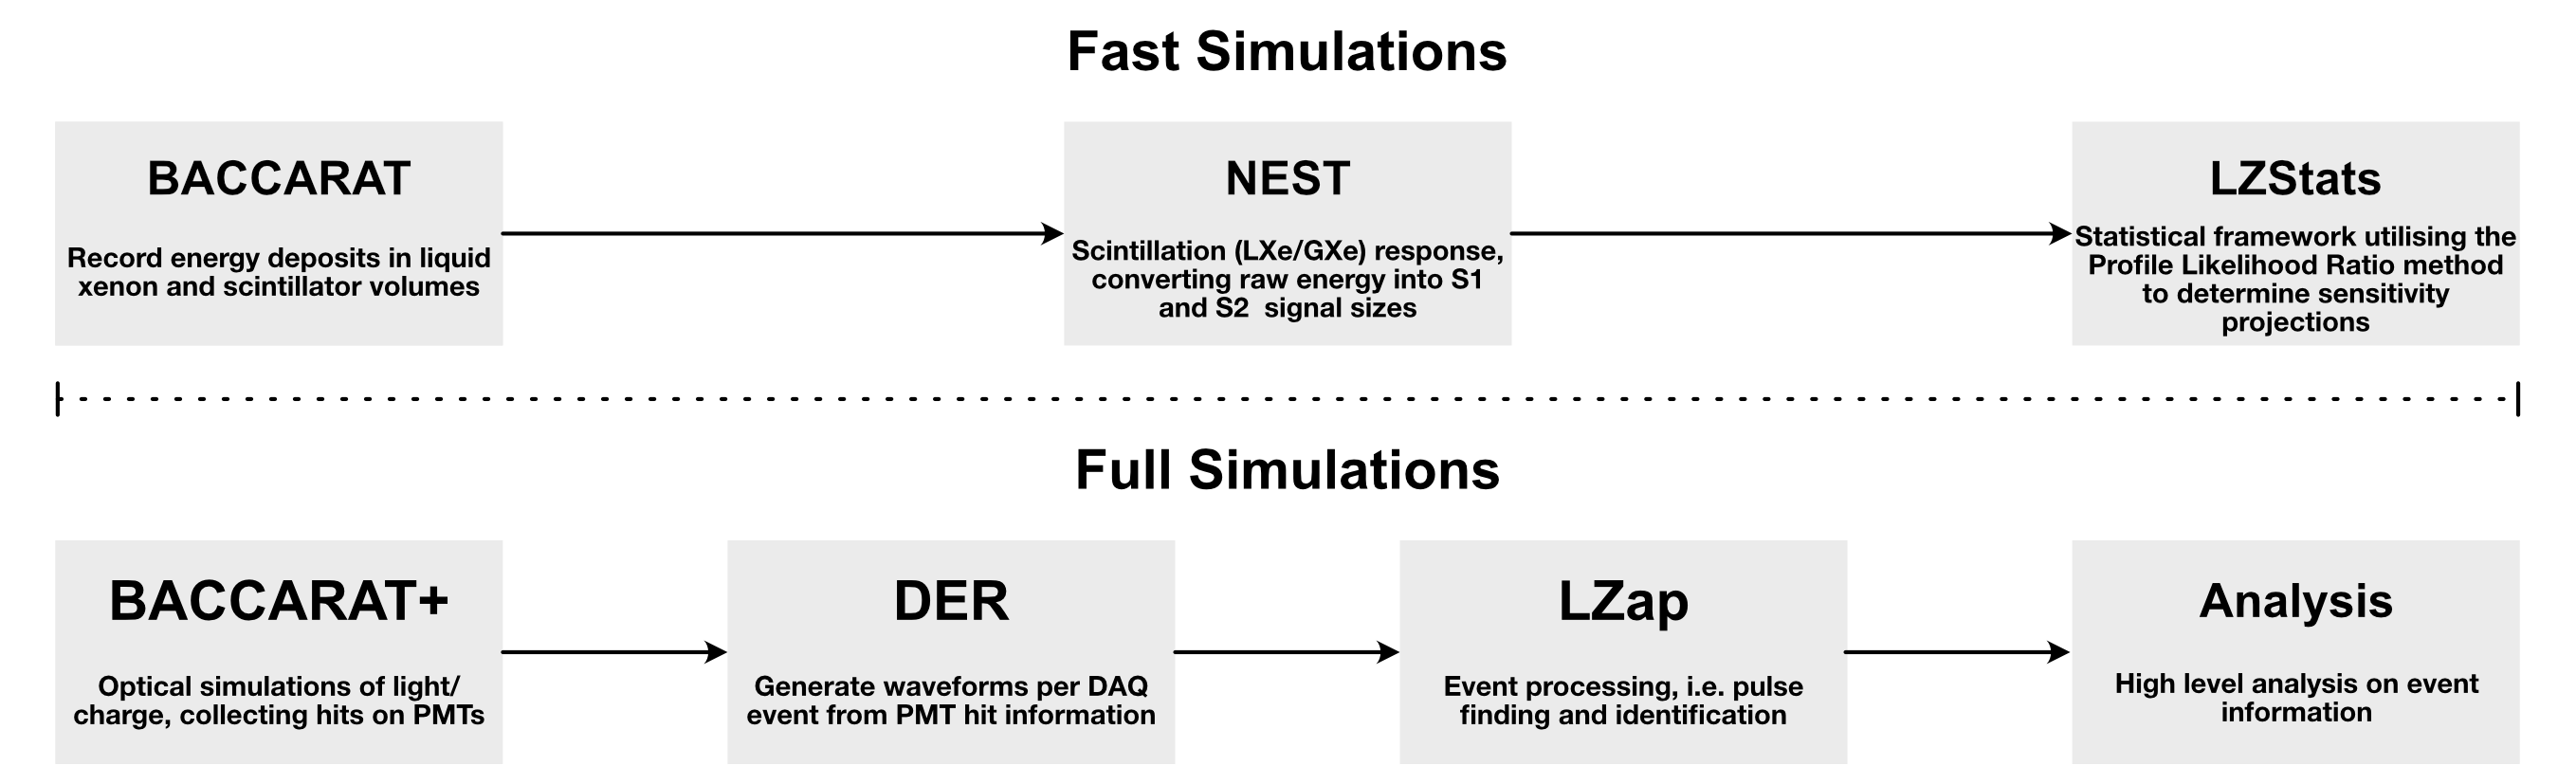
\includegraphics[scale=0.7]{Chapter_5/Figures/LZ_simulations_chains.png}
    \caption
    {The LZ simulation packages, detailing the fast and the full processing chains of background simulations. The fast chain is primarily used in sensitivity studies, whereas the full chain is used to generate ultra-realistic pulses for Mock Data Challenges (MDCs).}
    \label{fig:lz_simulation_chains}
\end{figure}
%

The fast simulation chain records energy depositions using \textsc{BACCARAT} and passes these depositions over to \textsc{NEST}, where the energy depositions are converted into S1 and S2 signals by using well understood light and charge yields in LXe, and applying detector-averaged quantities. In enabling fast generation of large datasets, this chain is often used in analysing background rates and informing sensitivity estimates. However, more minute details of events, such as, times of interaction and PMT photon hits are inaccessible. The full simulation chain includes the simulation of VUV photons and ionization electrons that are produced during xenon interactions, as well as the scintillation light generated in the skin and OD veto systems. Furthermore, a detector electronics response (DER) simulation is used to model the PMT response to VUV photons including quantum efficiency and dark noise, front-end and back-end electronics to generate realistic waveforms. These waveforms are saved are saved in realistic data structure to that of expected data---facilitating a training dataset used to prepare for real data through Mock Data Challenges (MDCs). These waveforms are passed through the LZ Analysis Package (LZap), which reconstructs pulse and event level information through a multitude of algorithms for data analysis.

The simulation studies highlighted in this chapter focuses predominantly on the fast simulation chain. The expected backgrounds from screening results are used as a bases to input into \textsc{BACCARAT}, where detector related background rates are determined. Dedicated particle generators are used to simulate surface and xenon contaminants; backgrounds from the cavern, cosmogenic muons and various physics backgrounds, such as solar, atmospheric and diffused supernova neutrinos. NEST is then used to generate background specific S1 and S2 signals that plug into the \textsc{LZStats} framework for the evaluation of sensitivity projections. The following sections will give a brief introduction to the fast simulation chain used in this work, a more in-depth highlight can be found in \cite{lz_simulations}. A description of \textsc{LZStats} framework and its statistical approach is detailed. Furthermore, projections made for the WIMP sensitivity of the LZ dark matter experiment and various other sensitivity studies, emphasising on the impact of the dominant radon background of LZ are presented.


%%------------------------------$$
\section{LZ Simulation Framework \& Detector Parameters}
\label{sec:LZ_simulation_framework}
%%------------------------------$$


\subsection{BACCARAT}
\label{secsec:BACCARAT}

\textsc{Geant4} is a toolkit used extensively in the nuclear and high-energy physics community to simulate the passage of particles and particle interactions through detectors and materials. The LZ simulation package \textsc{BACCARAT} is an extension to the simulation package developed for LUX \cite{AKERIB201263}, providing a more user-friendly interface to \textsc{Geant4} for low-background experiments. Simulations in low-background experiments differ to conventional particle colliders due to the origin of background sources. In low-background experiments, such as LZ, one of the main sources of background is embedded radioactive isotopes scattered throughout detector material; placing the source of radiation across a three-dimensional volume. Furthermore, every material and component within the detector has a unique radioactive composition; the simulation of which requires a collection of sources with potentially complicated spatial and radioactive extent.

\textsc{BACCARAT} is a simulation framework designed and used by LZ that takes a component-centric approach to event generation and recording. It implements a C++ detector component object that allows for spacial origin for radioactivity across a three-dimensional component or material for a more accurate modeling of impurities. Furthermore, each component can independently have a material specific recording level for the amount of information required, such as position, scattering information or energy deposition---significantly improving memory usage. The defined geometry of the LZ detector, illustrated on figure (\ref{fig:lz_geometry_viz}) relies heavily on \textsc{Geant4} classes.

%
\begin{figure}[b]
    \centering
    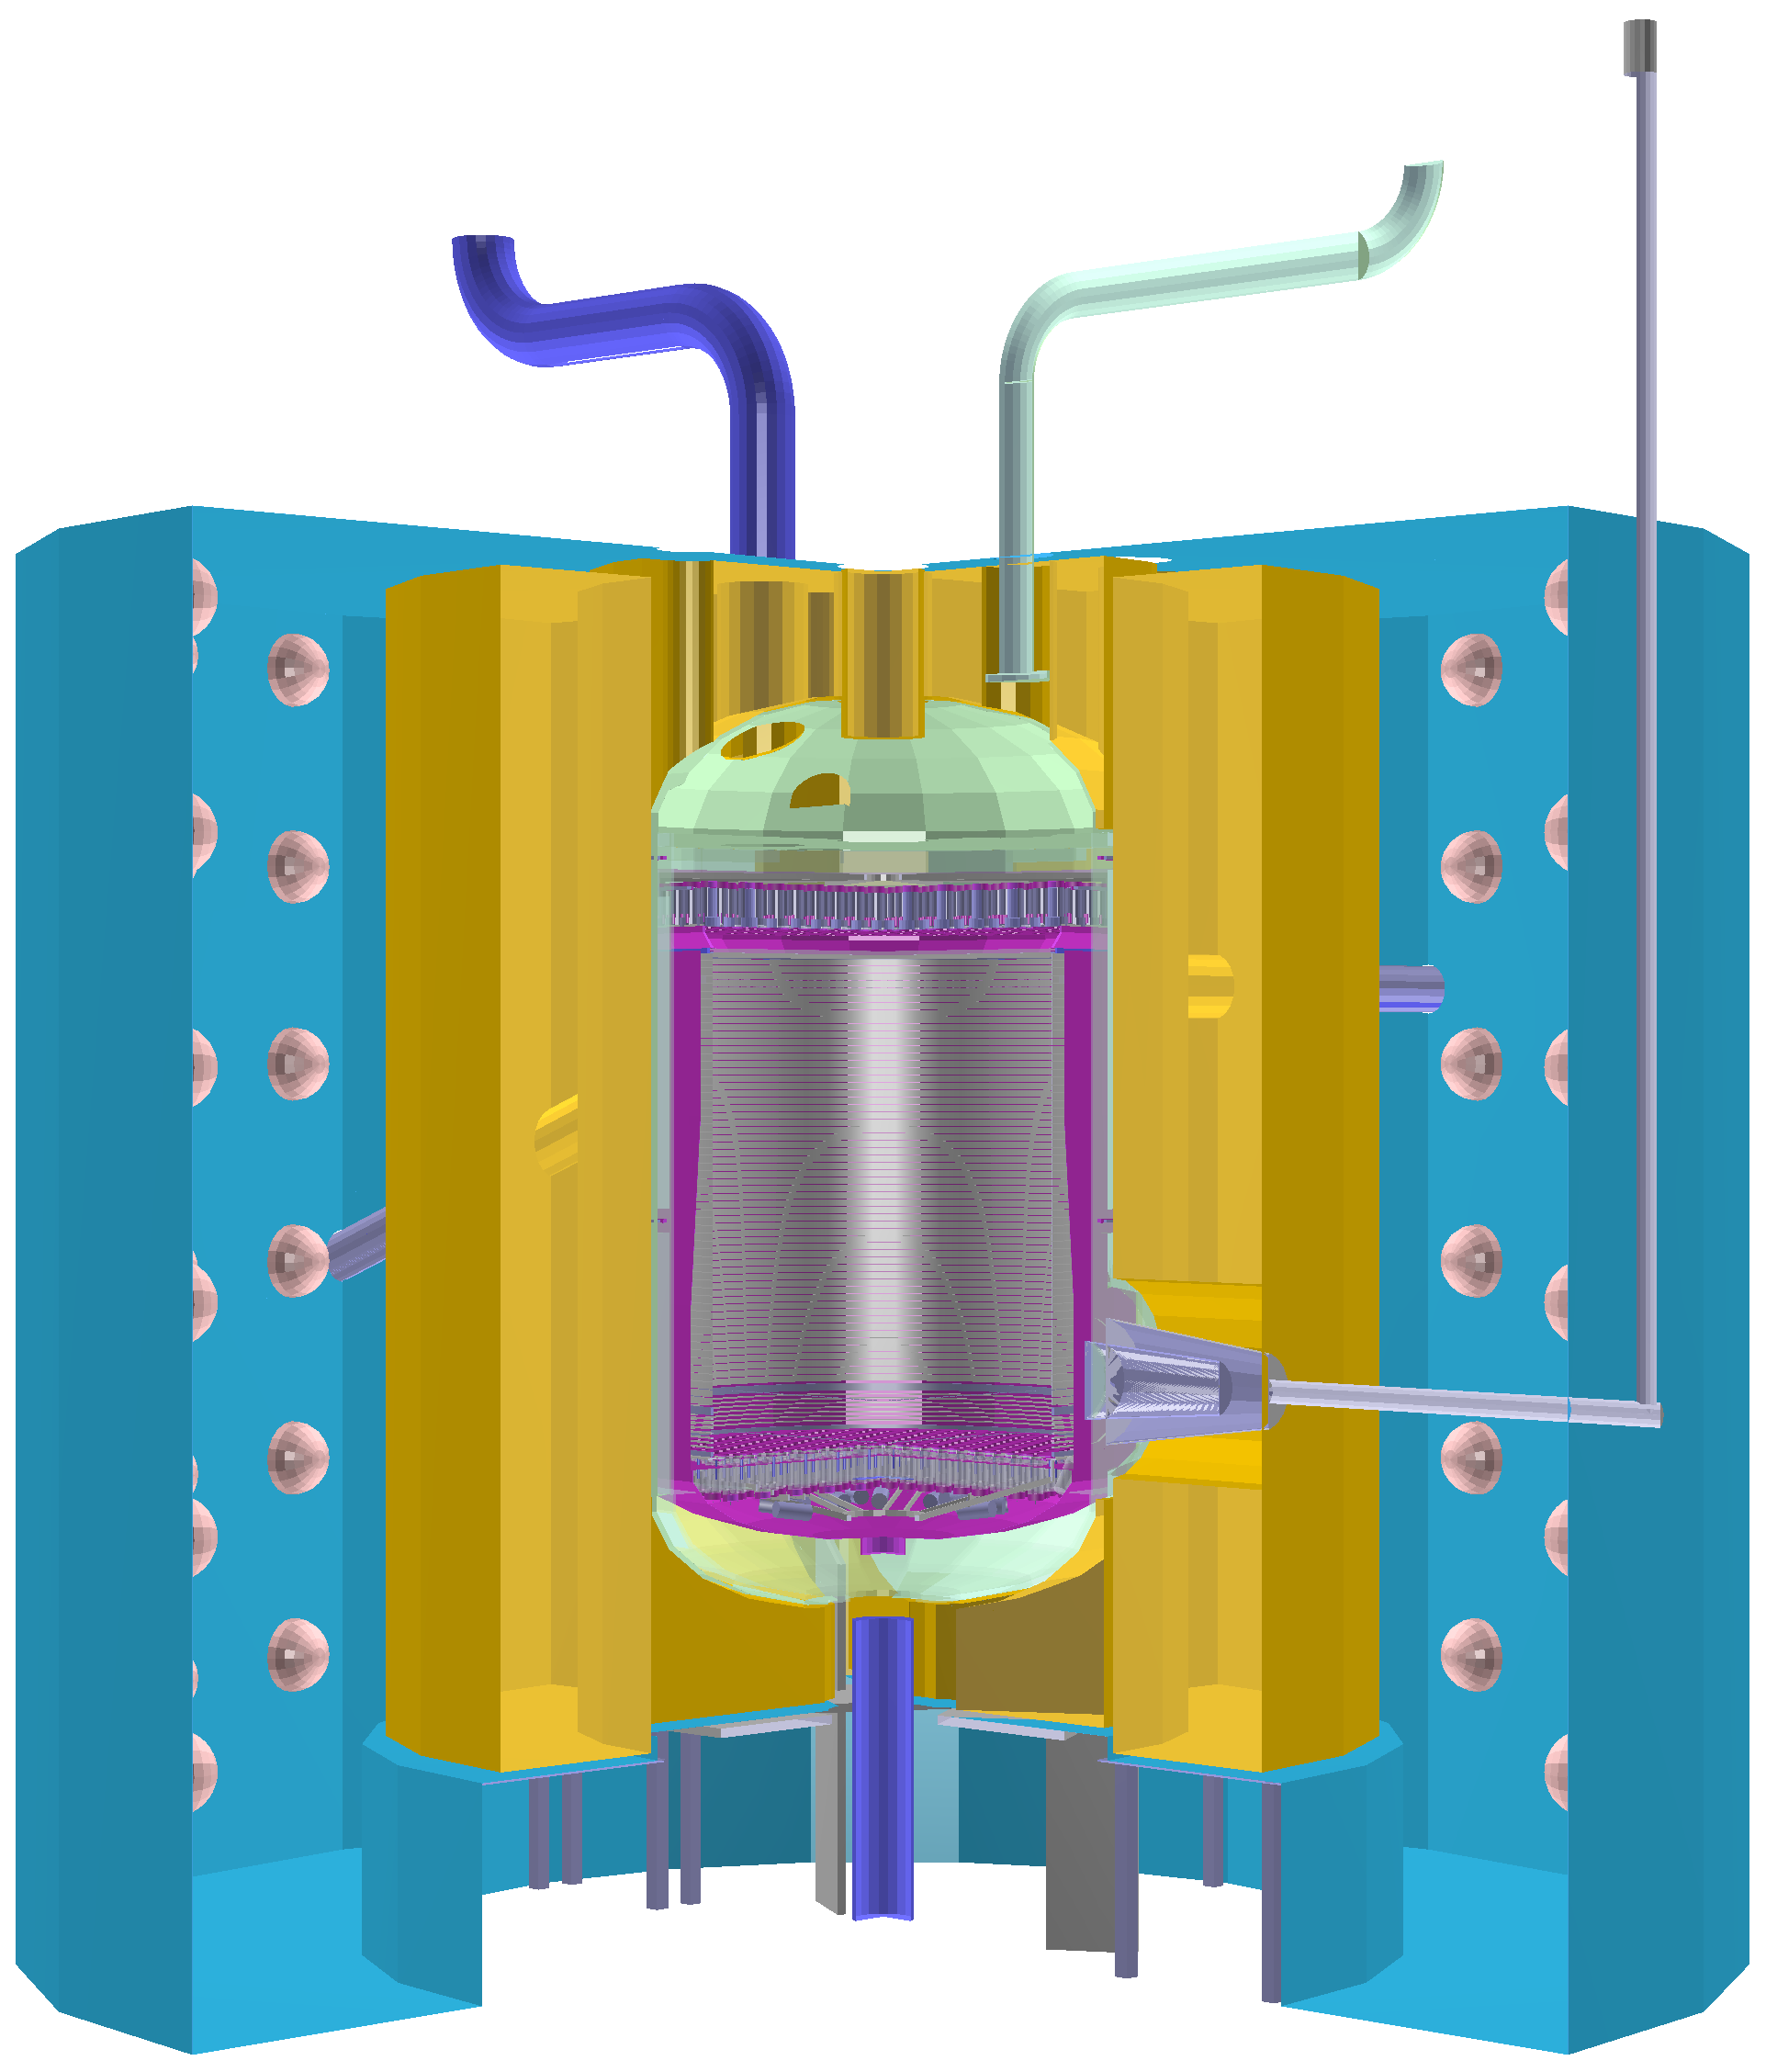
\includegraphics[scale=0.21]{Chapter_5/Figures/lz_geometry_viz.png}
    \caption
    {The geometry of the LZ detector as constructed by the \textsc{BACCARAT} simulation package illustrating some of the key components. The entire detector is immersed inside a water tank, with the inner part of the water tank shown in blue; holding the OD PMT structure, which face the GdLS outer detector tanks (yellow). The outer and the inner. cryostat (light green) holds the central TPC (magenta).}
    \label{fig:lz_geometry_viz}
\end{figure}
%

In modeling various physics processes, \textsc{BACCARAT} implements several modules that are contained in the \textsc{Geant4} toolkit, including \textit{G4EMLivermorePhysics}---covering electromagnetic interactions for \gamma{}-rays and electrons down to $\sim10$\,eV, where low energy processes, such as bremsstrahlung, the photoelectric effect, Rayleigh and Compton scattering are modeled \cite{osti_295438, osti_5691165}. Furthermore, when run in full simulation mode, \textsc{BACCARAT} implements a custom-built physics list (NEST) directly into the \textsc{Geant4} interface under \textit{G4S1Light} \& \textit{G4S2Light}, governing the detector specific generation of light and charge quanta in a xenon volume, respectively.

In addition to these, there are several other physics lists that have been implemented to simulate various other potential event topologies in LZ, such as, Cherenkov processes in non-xenon materials, rest and in-flight decay of radioactive nuclei via \alpha, $\beta{}^{\pm}$, \gamma-emission or electron capture; and relaxation of excited atomic states via the emission of X-rays and electrons. The \textsc{BACCARAT} physics list, particle generators and processes such as charge transport within xenon are continually improved for more realistic simulations. The code is maintained via an LZ inclusive Git repository and the studies highlighted in this chapter are with BACCARAT verified against \textsc{Geant4} version 10.3.


\subsection{NEST}
\label{secsec:NEST}

The NEST package introduced in section (\ref{subsubsec:light_charge}) plays a key role in the fast simulation chain. NEST is a semi-empirical collection of models, relying on data from multitude of past and present science and calibration datasets for \beta, \gamma and neutron-induced xenon recoils in varying electric fields, simulating the excitation, ionization, recombination, and electron electroluminescence processes in liquid or gaseous xenon. The previous versions of NEST \cite{Szydagis_2011, Mock_2014} modeled light and charge yields as a function of energy inspired by the Thomas-Imel box recombination model at low energies \cite{PhysRevA.36.614} and Doke modification to Birks’ law \cite{DOKE1988291} at high energies, with coefficients as functions of field. The version used as part of this study, v2.0, uses a range of sigmoidal-class functions to model yields as functions of energy \cite{nest_v2}. The yields are readily modeled as a function of particle and interaction type, energy, ionisation density, electric field and fluid density.

The output from \textsc{BACCARAT}; information on energy deposition, material media, type of interaction, is fed into NEST for a rapid conversion into the detector observable quantities. The conversion from deposited energy to detector observables (S1 \& S2) is calculated in multiple steps, where the exciton-to-ion ratio is first considered to determine the amount of excitons, leading to primary scintillation (S1) and electron-ion pairs. Energy-specific recombination probabilities are then applied to determine the amount of electron-ion recombination, resulting in a reduction in S2 signal, but an increase in S1. For processes where energy is lost through heat; i.e., nuclear recoil events, a simple power law approximating the Lindhard factor is applied \cite{Lindhard, Lindhard_2}. The transportation of escaped electrons to the liquid-gas interface is handled by NEST through a parametrised electric field applying diffusion and a finite mean free path; where upon reaching this barrier, an extraction efficiency is applied through probabilistic quantities dependent on extraction field strength in the gas phase. The resulting output from NEST then takes into account detector specific quantities to produce a corrected S1$_{c}$ and S2$_{c}$ signal in \textit{photons detected} (phd).


\subsection{Detector Parameters}
\label{secsec:detector_param}

%
\begin{table}[b!]
\centering
\caption
[Key detector parameters for the LZ experiment.]
{Key detector parameters for the LZ experiment. PDE refers to \textit{photon detection efficiency}, SE to \textit{single electron}, e to \textit{electron}, ph and phd to \textit{photon} and \textit{photons detected}, respectively.}
\label{tab:lz_parameters}
\vspace{1mm}
\renewcommand{\arraystretch}{1.2}
    \begin{tabularx}{0.7\linewidth}{@{\extracolsep{\fill}}lll}
    \toprule
    \textbf{Detector Parameter} & %1
    \textbf{Value} & %2
    \textbf{} & %3
    \hline
    \hline

    Drift electric field                        & 310 & V/cm \\
    Electron lifetime                           & 850 & \micro{}s \\
    Electron extraction efficiency              & 95 & \% \\
    Average PMT efficiency                      & 27 & \% \\
    Average PDE in liquid (\textit{g$_{1}$})    & 0.119 & phd/ph \\
    Average PDE in gas (\textit{g$_{1gas}$})    & 0.102 & phd/ph \\
    Single electron size                        & 83 & phd \\
    Effective charge gain (\textit{g$_{2}$})    & 79.2 & phd/e \\
    S1 coincidence level                        & 3 & ph \\
    Single phe trigger efficiency               & 95 & \% \\
    PTFE reflectivity in LXe                    & 97.7 & \% \\
    PTFE reflectivity in GXe                    & 85 & \% \\ 
    
    \bottomrule
    \end{tabularx}
\end{table}
%

The detector parameters that are key in determining the actual observed signal for \textit{S1, S2, x-y-z}, from the point of interaction and through the physical and electrical processes of LZ are summarised in table (\ref{tab:lz_parameters}). Once an event occurs within the LXe volume, the photons that are produced---referred to as raw S1---traverse the volume, reflecting off of the PTFE walls before hitting a PMT successfully. The $g_{1}$ factor, formally known as the photon detection efficiency in the liquid represents the averaged successful recording of a single photon, taking into account reflectively and PMT quantum efficiencies; $g_{1gas}$ is the equivalent detection efficiency for S2 electroluminescence photons generated in the gaseous extraction region. The current estimates derived from optical simulations based on reflectively measurements of the LZ PTFE \cite{Neves_2017, Haefner_2017} for $g_{1}$ and $g_{1gas}$ are 0.119 phd/ph and 0.102 phd/ph, respectively. These values include considerations of 3'' Hamamatsu PMT quantum efficiency, double photoelectron emission probabilities \cite{L_pez_Paredes_2018}, first dynode collection efficiency and photon absorption length in LXe motivated by the literature \cite{lux_signal_yields}. Single electron size represents the average number of photons detected per extracted electron, whereas the photons detected from a raw S2 signal is represented by the $g_{2}$ factor. $g_{2}$ takes into account the extraction efficiency at the liquid-to-gas boundary, adding an averaged correction for the lost electrons, resulting in an effective charge gain of 79.2 phd/e.

The detector parametrisation factors detailed in table (\ref{tab:lz_parameters}) are evaluated alongside the \textsc{BACCARAT} input to the \textsc{NEST} framework in calculating corrected detector observable signals, S1$_{c}$ and S2$_{c}$. Although this process takes certain parameters as their averaged representations; excluding differences arising from event location, or PMT specific divergences on an event-to-event bases; it allows for fast generation of (S1$_{c}$, S2$_{c}$) probability density functions (PDF) that are representative of detector operational conditions. The PDFs of background and signals events are then fed into the LZ statistical framework, \textsc{LZStats}, for sensitivity studies. The event selection criteria and the representative background rates under projected operational conditions, as determined by the use of the LZ simulation framework are detailed in the next section.   



%%------------------------------$$
\section{Background Projections for WIMPs}
\label{sec:uclradon}
%%------------------------------$$

The LZ detector is capable of detecting signals from a wide spectrum of event topologies and energy ranges. This wide range of energy-space is made accessible by exploiting the two signal types in LZ, measurement of scintillation light and charge production, in various search types; i.e. S2-only, S1-S2 and S1-only searches. At sub-keV energies, S2-only searches are used to probe for lighter WIMP, sub-geV hidden sector and asymmetric dark matter models. Low energy depositions at this regime usual result in free electrons extracted without any accompanying S1 signal. At much higher energies, LZ is capable of detecting the \XeOTS{} \neutrinolessDoubleBeta{}-decay with a $Q_{\beta \beta}$ value of 2458 keV \cite{Akerib_2020_double_beta}.

The observation of a WIMP signal is conducted in the S1-S2 space in the LZ detector, coming from an excess of single-scatter nuclear recoil events taking place within a WIMP centric fiducial volume and a pre-defined energy region of interest (ROI), optimised for the signal-to-background ratio. The full ROI can be seen as a selection of detector-specific cuts applied to the outcome of the Monte Carlo simulations, which are dictated by measured material radioactivity and anticipated levels of dispersed and surface radioactivity. The following sections will highlight the WIMP search event selection criteria used for constructing the background model for the sensitivity projections, and present the integrated background rate for ER and NR counts in the 5.6 tonne fiducial mass for a 1000 live day run using a reference cut-and-count analysis; which was used for the purpose of tracking material radioactivity throughout the design and construction phase of the LZ experiment. The full RIO highlighted below is relevant for the PLR analysis, detailed in section (\ref{sec:lz_stats}), and used to calculate the sensitivity and the discovery potential for WIMPs using the LZ detector.


\subsection{Background Selection Cuts}
\label{secsec:background_selection}

In the design and construction phase of the detector, the attribution of specific backgrounds to planned operational conditions and material radioactivity is vital in selecting the most appropriate materials and the final design of the experiment. Analysis of simulation results are used to determine the total number of background events and their distribution in the S1$_{c}$--S2$_{c}$ space, from which PDFs are generated for the PLR analysis. A set of cuts is applied to the simulated data to select WIMP-like events and determine the impact of backgrounds on the WIMP-search analysis. These cuts, which are aimed at imitating those that will be applied to real WIMP search data are as follows:

\begin{itemize}
  \item Region of interest---\textbf{RIO}: Defines the energy window of the expected WIMP-like events in LXe. Backgrounds of interest for the WIMP search are those that fall into this energy region of interest.
  
  \item Single scatter--\textbf{SS}: Requirement of the energy deposition taking place in a single spacial (\textit{}x-y-z}) coordinate within expected detector resolution. 
  
  \item Skin veto--\textbf{Skin}: Rejection of events in the active volume if an accompanying event occurring in the skin region.
  
  \item Outer detector veto--\textbf{OD}: Rejection of events in the active volume if an accompanying event occurring in the outer detector.
  
  \item Fiducial Volume--\textbf{FV}: The virtual volume within the active LXe TPC that an event is required to take place. This volume is defined to remove the overwhelming background from the walls of the TPC.
\end{itemize}

The region of interest for WIMPs is defined both in energy-deposited terms, i.e. in keV and in detector observable terms, S1-S2. In the energy space, where deposit-only simulations are considered without the implementation of NEST, this window is given as 1.5--6 \kevee{} for ERs and 6--30 \kevnr{} for NRs. The difference between these energy terms is to represent the quenching that takes place for an NR event. The conversion between these two representative energy depositions is given by, 
%
\begin{equation}
    &E_{dep}(keV_{ee}) = E_{ER} + \frac{1.5}{6.0} E_{NR} \\
    \vspace{2mm}
    &E_{dep}(keV_{nr}) = E_{NR} + \frac{6.0}{1.5} E_{ER}.
    \label{eq:kev_ee_nr}
\end{equation}
%

The energy scale used is dependent on the type of simulated background; i.e. \beta and \gamma interactions are represented by \kevee{}, whereas nuclear recoil interactions are given as \kevnr{}. In real data, there is no definite way to distinguish ER from NR events, hence interactions are usually represented in one or the other version. To better replicate the real impact of the detector on energy depositions and to simulate the treatment of real data, the ROI is also defined in terms of S1 and S2 space. In this space, the WIMP ROI is defined by 0 < S1$_{c}$ < 80 phd, with a 3-fold S1 coincidence requirement within the TPC PMTs. The 3-fold cut is required to reduce background events leaking into the WIMP ROI from coincidences between PMT dark noise and S2-only events. In addition, the S2-raw signal is required to be greater than 420 phd---equivalent to $\sim5$ extracted electrons. This is to ensure an adequate S2 size for an accurate \textit{x-y} position reconstruction, reducing backgrounds due to misreconstruction of events into the fiducial volume.

Single scatter events are those that deposit all of their energy into a single interaction point, as expected from a WIMP interaction. Although on microscopic scales, total energy deposition of background events may result from many micro-depositions taking place within a very small radial regime, these interactions cannot be resolved due to the expected spatial resolution of the detector. A single scatter cut placed on the energy-weighted standard deviation ($\sigma_{r}$ \& $\sigma_{z}$) is therefore used to reject multi-scattering neutrons and \grays{} that falls outside of the energy-weighted clustering resolution. The energy weighted mean position is defined as, 
%
\begin{equation}
    \big\langle r_{E} \big\rangle = \frac{\sum_{i}E_{i}r_{i}}{\sum_{i}E_{i}} \;\;\;\;\; \big\langle z_{E} \big\rangle = \frac{\sum_{i}E_{i}z_{i}}{\sum_{i}E_{i}},
    \label{eq:weighted_mean_position}
\end{equation}
%
where $r_{i}$ and $z_{i}$ represent the radial and vertical interaction points and $E_{i}$, the energy deposited into each vertex. The energy-weighted standard deviation ($\sigma_{z}$ \& $\sigma_{r}$) is then given by,
%
\begin{equation}
    \sigma_{r} = \sqrt{\frac{\sum_{i}E_{i}(r_{i} - \big\langle r_{E} \big\rangle)^{2} \times \sum_{i}E_{i}}{(\sum_{i}E_{i})^{2} - \sum_{i}E_{i}^{2}}} \;\;\;\;\; \sigma_{z} = \sqrt{\frac{\sum_{i}E_{i}(z_{i} - \big\langle z_{E} \big\rangle)^{2} \times \sum_{i}E_{i}}{(\sum_{i}E_{i})^{2} - \sum_{i}E_{i}^{2}}}.
    \label{eq:energy_weighted_sd}
\end{equation}
%
The single scatter requirements used in the background selection of LZ simulations is developed through taking into account the PMT size and the array layout, and by incorporating previous LUX position reconstruction studies \cite{Akerib_2018_lux_position}. A conservative requirement of $\sigma_{r}$ < 3.0 cm and $\sigma_{z}$ < 0.2 cm is set for S2 signals at the detection threshold. Position resolution in real LZ data will make use of hit patterns and waveform shapes, and is expected to be < 1 cm radially and to vary with energy and radial position. 

In addition, events occurring in the active volume of the TPC with a time-coincident event taking place within the skin or the outer detector veto system is also rejected. For the LXe skin veto, at least 3 phd must be observed within an 800 \micro{}s coincidence window, either before or after the TPC S1 signal. Whilst for the OD, a minimum of 200 keV must be deposited within a 500 \micro{}s interval. The primary purpose of the veto systems is to ensure the vetoing of both prompt \gamma and delayed signals from thermal neutron capture.

%
\begin{figure}[b]
    \centering
    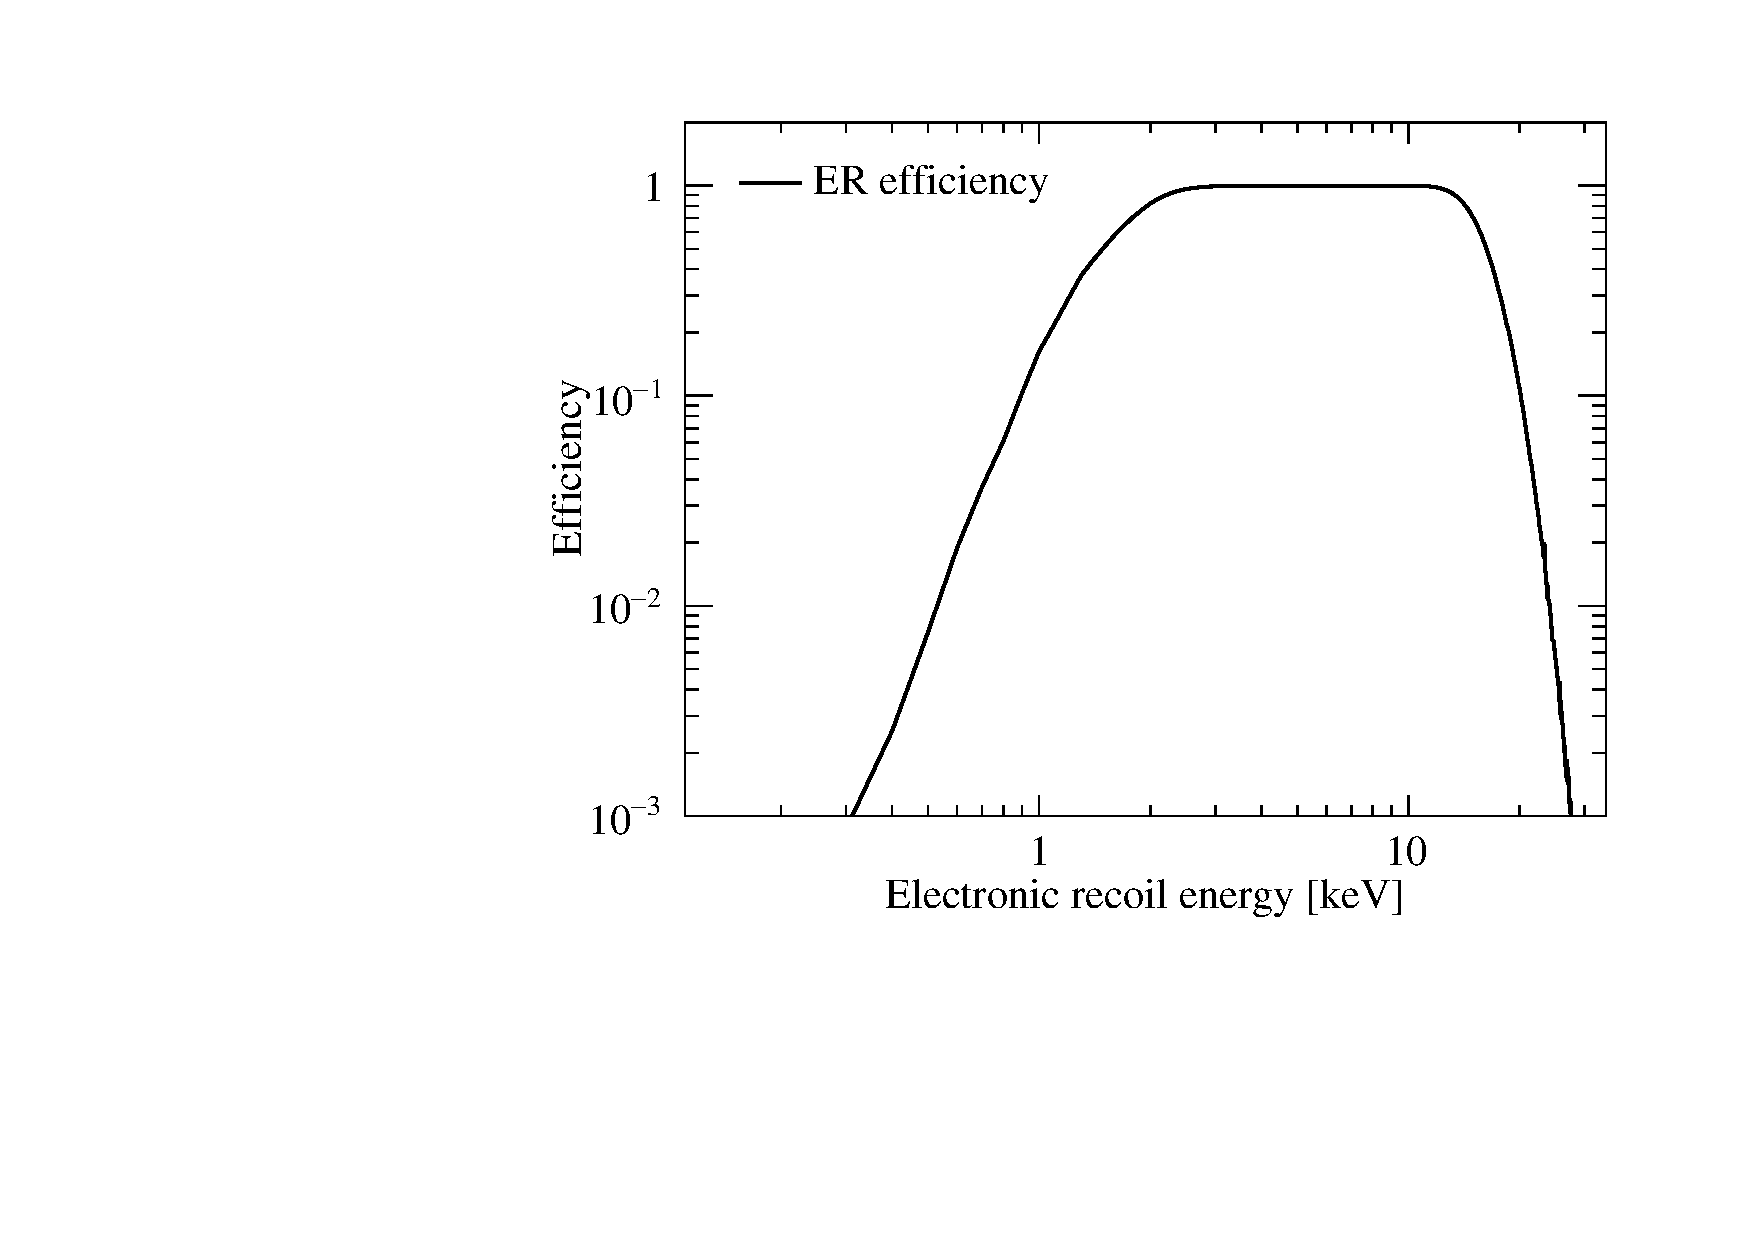
\includegraphics[scale=0.39]{Chapter_5/Figures/er_efficiency.pdf}
    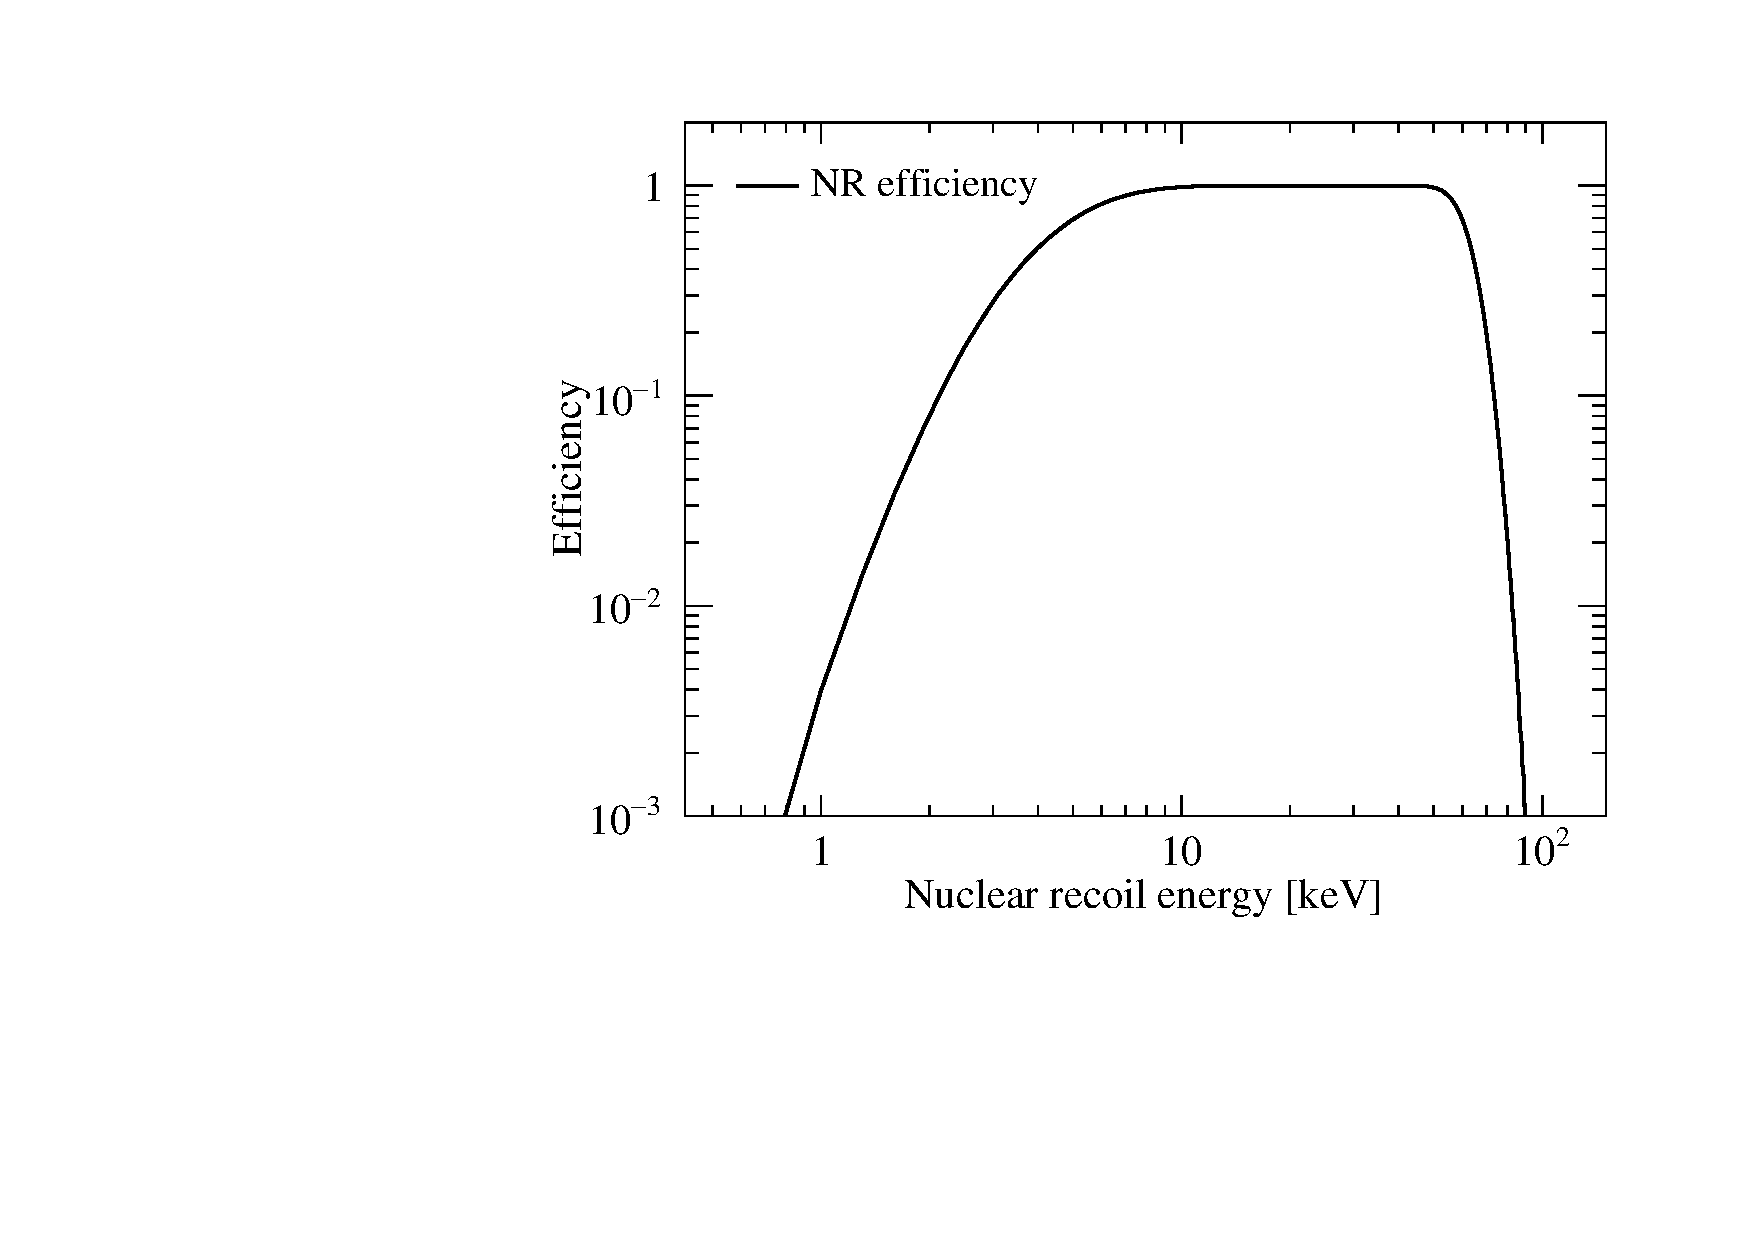
\includegraphics[scale=0.39]{Chapter_5/Figures/nr_efficiency.pdf}
    \caption[Simulated efficiency for electronic (left) and nuclear recoil (right) events after the application of the WIMP ROI event selection cuts.]%
    {Simulated efficiency for electronic (left) and nuclear recoil (right) events after the application of the WIMP ROI event selection cuts. These cuts include the 3-fold S1 coincidence, S1$_{c}$ < 80 phd and S2 > 420 phd. Figure adapted from \cite{akerib2018projected}.}
    \label{fig:lz_er_nr_efficiency}
\end{figure}
%

Lastly, the final crucial event selection criteria is the fiducial volume cut. This cut is designed to remove events near the edge of the TPC. A cylindrical virtual volume with boundaries defined to be 4 cm from the TPC walls, 2 cm above the cathode grids (with 14.8 cm of LXe below the cathode providing further shielding) and a further 13 cm below the gate grid. This volume contains a total of 5.6 tonnes of LXe and is largely motivated by the misreconstructed wall events leaking into the FV. This leakage probability has previously been studies by using the Mercury algorithm---which is responsible for the \textit{x-y} reconstruction from S2 PMT hits---and shown to be less than $10^{-6}$ for the smallest S2 signals at 4cm away from the walls, ensuring that wall events are a sub-dominant background \cite{Solovov_2012, Akerib_2018_lux_mercury}. Simulated efficiencies after the application of the WIMP RIO cuts as a function of recoil energy for electronic and nuclear recoils is shown in figure (\ref{fig:lz_er_nr_efficiency}}.


\subsection{Projected Background Rates}
\label{secsec:background_table}

During the construction phase of the detector, a cut-and-count style analysis was performed on the simulated background dataset as a means of assessing the impact of design specific decision making. The integrated rates calculated for the ER and NR backgrounds were selected using the WIMP RIO in the energy-space, where ER events between 1.5–6.5 keV and NR events between 6–30 keV were selected in a full 1000 live day run with a 5.6 tonne fiducial mass. Although the analysis takes a different approach to that used by the PLR analysis, it nevertheless provides an insight into the rates expected for the WIMP search and in informing design specifications. The analysis simulates many of the background detailed in section (\ref{sec:background_origins}) and various other event types that contribute towards the integrated background rate; such as physics backgrounds from astrophysical neutrinos. The contributions from the most relevant background components are listed in table (\ref{tab:lz_background_count}), with the expected ER and NR counts for each entry. 

Background events from \textit{detector components} originate from naturally occurring radioactive isotopes found within the construction material of the experiment. Isotopes of interest for simulations are the decay chains of \UTTE{}, \UTTF{}, \ThTTT{}; as well as, \gamma-emitting isotopes of \KFZ{}, \CsOTS{} and \CoSZ{}. The results from the comprehensive screening campaign of LZ (> 1200 assays over 5 years) are used quantify the activity of such isotopes within the component-centric BACCARAT framework. Due to the selective material sourcing process used by LZ, backgrounds from detector components are sub-dominant. Furthermore, isotopic \textit{surface contamination}, through dust deposition (500 ng/cm\squared{}) and \RnTTT{} plate-out (50 nBq/cm\squared) leads to both ER events near the detector surface and NR events from \alphaN{} processes. Although a significant amount of wall events are rejected by the fiducial volume cut, some make it into this volume due to algorithmic spatial misreconstruction near the walls and mobility of \BiTOZ{}. Wall backgrounds have been a huge focus during construction with extensive surface cleanliness protocols in place as detailed in section (\ref{subsec:surface_contaminants}), thus the assumptions used in this study are expected to be conservative.

%
\begin{table}[]
\centering
\caption{Estimated background rates from all significant contributors in a 1000 live day run and a 5.6 tonne fiducial mass. The ER and NR counts are from a region of interest relevant to a 40 GeV/c\squared{} WIMP; approximately 1.5--6.5 keV for ERs and 6--30 keV for NRs; and after application of the single scatter, skin and OD veto cuts. Counts from the solar \BE{} and hep neutrinos are given as a reference, as they are not significant above an NR energy of 6 keV. The ER discrimination is a conservative value taken from the LZ TDR \cite{lz_tdr}, aimed at selecting events from the energy-space that is most relevant for NR interactions.}
\label{tab:lz_background_count}
\vspace{1mm}
\renewcommand{\arraystretch}{1.2}
    \begin{tabularx}{1.0\linewidth}{@{\extracolsep{\fill}}lll}
    \toprule
    \textbf{Background Sources} & %1
    \textbf{ER} & %2
    \textbf{NR} & %3
    \hline
    \hline

    Detector components                         & 9    & 0.07 \\
    Surface contamination                       & 40   & 0.39 \\
    Laboratory and cosmogenics                  & 5    & 0.06 \\
    \textbf{Dispersed radioisotopes (Xenon)}    &      &      \\
    \RnTTT{} (1.8 \micro{}Bq/kg)                & 681  & 0    \\
    \RnTTZ{} (0.09 \micro{}Bq/kg)               & 111  & 0    \\
    \XeOTS{} ($2\nu\beta\beta$)                 & 67   & 0    \\
    \KrEF{} (0.015 ppt g/g)                     & 24.5 & 0    \\
    \ArTN{} (0.45 ppb g/g)                      & 2.5  & 0    \\
    \textbf{Astrophysical neutrinos}            &      &      \\
    Atmospheric (Atm)                           & 0    & 0.46 \\
    Diffuse supernova (DSN)                     & 0    & 0.05 \\
    Solar (\BE{} + \textit{hep})                & 0    & 38*  \\
    Solar (\textit{pp} + \BeS{} + \NOT{})        & 191  & 0    \\
    \hline
    Total                                                       & 1131 & 1.03 \\
    Total (with 99.5\% ER discrimination, 50\% NR efficiency)   & 5.66 & 0.52 \\
    
    \bottomrule
    \end{tabularx}
\end{table}
%

Environmental backgrounds either generated from cosmogenic activation or originating from the surrounding environment of the detector are combined under \textit{laboratory and cosmogenics}. The ER background from this source is predominantly from \gamma-ray events from the rock, as detailed in section (\ref{sec:external_backgrounds}); with a slight contribution from activation products \XeOTS{} and \ScFS{}. The NR background is from muon-induced neutrons. 

Although xenon is mostly radiopure, there are trace amounts of internal and external contaminants that contribute strictly in the ER band of the background spectrum. The dominant internal background comes from the $2\nu\beta\beta$ of \XeOTS{}, which exists in trace amounts within the sourced xenon. Xenon usually contains other isotopes, such as \KrEF{} and \ArTN{}. These isotopes are remnants from the production of xenon. The concentration of these isotopes provided in table (\ref{tab:lz_background_count}) are estimated based on the expected performance of the a custom-made gas chromatography system designed and installed at SLAC to remove krypton \cite{lz_tdr}. The krypton requirement is extraordinarily ambitious, hence sensitivity studies using 0.30 ppt g/g concentrations have also been performed to quantify the impact. The largest contributor from xenon contaminants is the backgrounds originating from radon emanation. The ER contributions from \RnTTT{} and \RnTTZ{} account to a total of 792 events---equivalent to $\sim70\%$ of all ER backgrounds from the cut-and-count analysis. This is based on a uniform \RnTTT{}(\RnTTZ{}) activity of 1.8(0.09) \micro{}Bq/kg; which falls within the bounds of the optimistic and the conservative projections from section (\ref{LZ_radon_diagram_paper}).

The last major background contribution to the WIMP search ROI is from \textit{astrophysical neutrinos}. The elastic neutrino-electron scattering \cite{HASERT1973138} and coherent elastic neutrino-nucleus scattering (CE$\nu$NS) \cite{Akimov_2017} are the two main interaction types, leading directly to ER and NR events, respectively. There are several sources of neutrino backgrounds observed by the LZ detector; atmospheric neutrinos produced in muon and pion decays, neutrinos produced in distant supernovae events, and solar neutrinos originating from various fusion reactions within the sun. The solar neutrino background for WIMP masses greater than $\sim20$ GeV/c\squared{} is dominated by \textit{pp} neutrinos, with contributions from the \BeS{} and CNO (Carbon-Nitrogen-Oxygen) cycles. The observed rates from elastic neutrino-electron scattering leading to ER events in LZ are calculated using flux and spectra from \cite{Bahcall_2004}, incorporating up-to-date oscillation parameters from \cite{Patrignani:2016xqp}. To take into account the effect of atomic binding, a scaling factor based on the relativistic random phase approximation calculation in \cite{Chen_2017} is applied to the free electron scattering rate below 30 keV. The \BE{} and hep neutrino rates are only relevant for NR energies $\lesssim 6$ keV, equivalently for WIMP masses below $\sim20$ GeV/c\squared{}. At this regime, CE$\nu$NS of neutrinos originating from the two fusion processes,
%
\begin{equation}
    ^{8}\MathText{B} \;\; &\rightarrow \;\; ^{7}\MathText{Be}^{*} \; + \; \MathText{e}^{+} + \nu_{e} \;\;\; (^{8}\MathText{B} \;\; neutrinos) \\
    ^{3}\MathText{He} + p \;\; &\rightarrow \;\; ^{4}\MathText{He} \; + \; \MathText{e}^{+} \; + \; \nu_{e} \;\;\; (hep \;\; neutrinos),
    \label{eq:solar_neutrino_generation}
\end{equation}
%
become dominant irreducible NR backgrounds. Although table (\ref{tab:lz_background_count}) provides a reference event rate for \BE{} and \textit{hep} neutrinos, they do not contribute to the total cut-and-count rate observed for a 40 GeV/c\squared{} WIMP; nevertheless, they are included in the WIMP sensitivity calculations using the full PLR treatment described in section (\ref{sec:lz_stats}).

The cut-and-count analysis for a 40 GeV/c\squared{} WIMP results in a total of 1131 ER events and 1.03 NR events, prior to ER--NR discrimination. In applying a 99.5\% discrimination selection on ER events as described in figure (\ref{fig:er_nr_discrimination}) and a 50\% NR efficiency; the total sum of irreducible backgrounds in the signal region result in 6.18 events in a 1000 live day run within a 5.6 tonne fiducial volume. The spectral contributions from the background sources highlighted in table (\ref{tab:lz_background_count}) for NR and ER events are shown in figures (\ref{fig:lz_nr_spectrum}, \ref{fig:lz_er_spectrum}), respectively. These figures show spectral rates of single scatter events in the fiducial volume, excluding the energy RIO, skin, OD cuts to provide a wider picture of background rates. The S1--S2 PDFs are a bi-product of the rates shown here, after the application of WIMP-specific ROI cuts and are used as an input to the \textsc{LZStats} framework for sensitivity studies.

%
\begin{figure}[h]
    \centering
    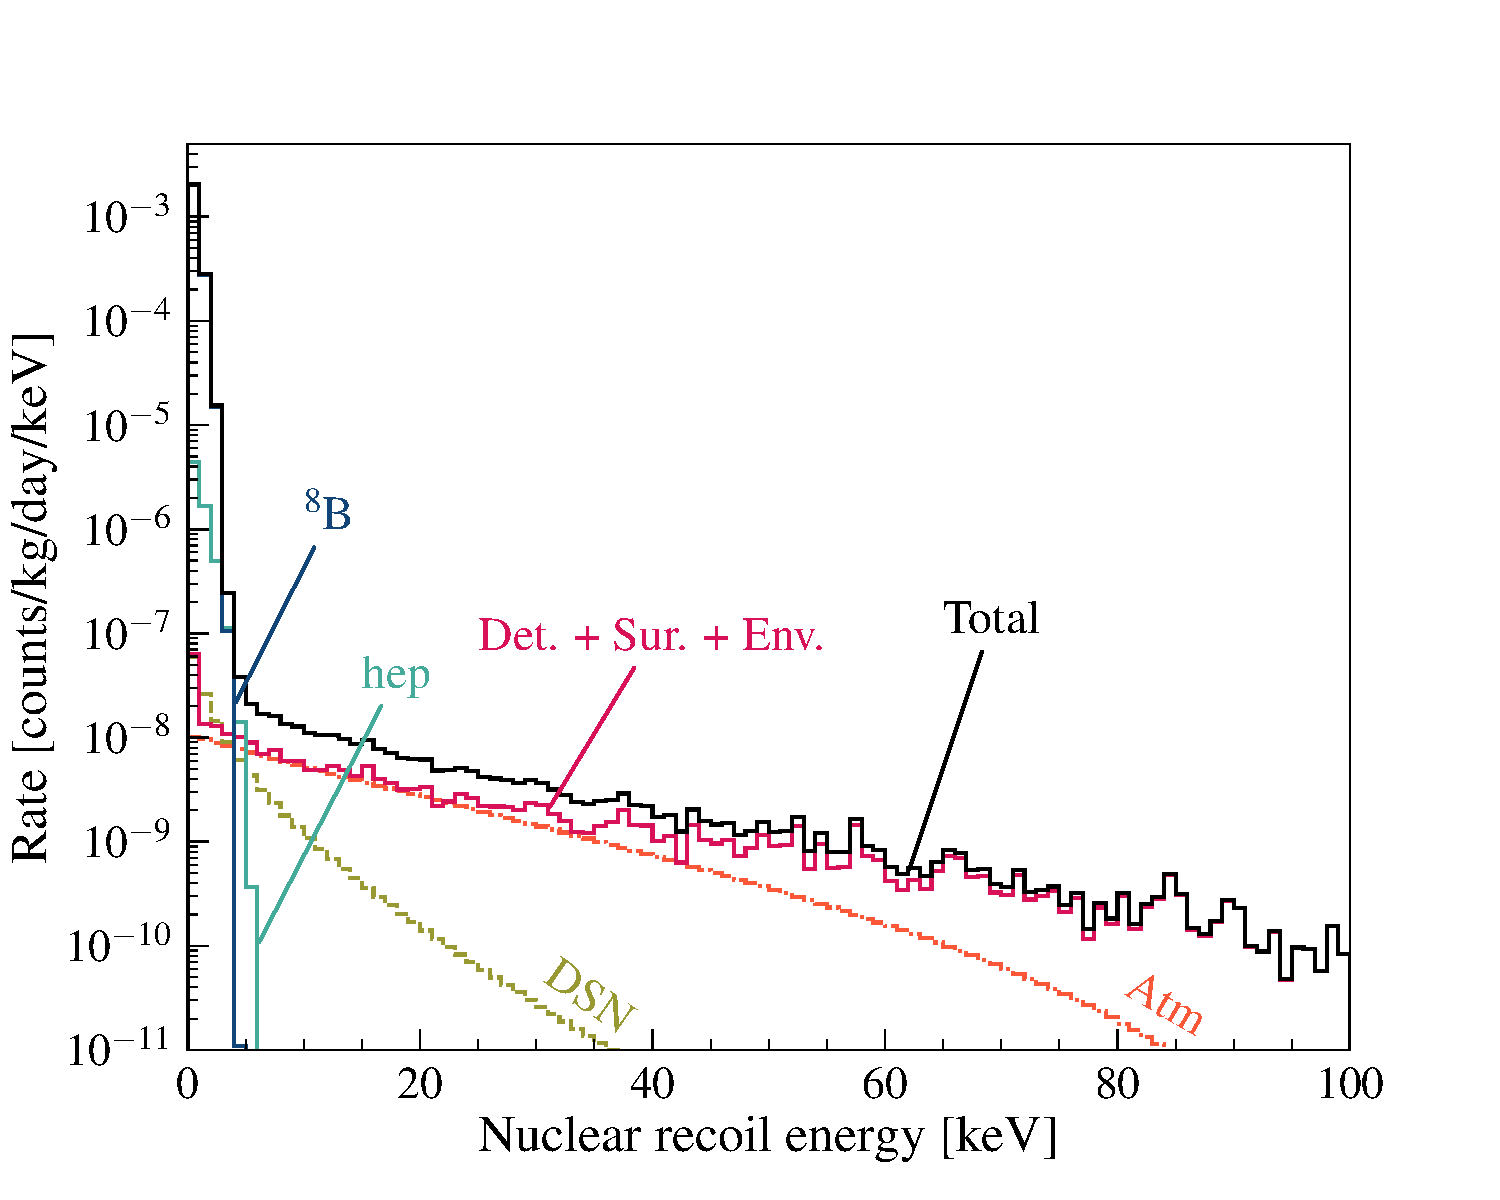
\includegraphics[scale=0.5]{Chapter_5/Figures/nr_background_spectrum.pdf}
    \caption[The projections of NR background spectra in the 5.6 tonne fiducial volume for single scatter events, including the skin and OD veto cuts.]%
    {The projections of NR background spectra in the 5.6 tonne fiducial volume for single scatter events, including the skin and OD veto cuts. Detector efficiency and WIMP-RIO cuts on S1$_{c}$ are also excluded. Laboratory, cosmogenic and surface backgrounds are combined together as (Det. + Sur. + Env.). Figure adapted from \cite{akerib2018projected}.}
    \label{fig:lz_nr_spectrum}
\end{figure}
%

%
\begin{figure}[t!]
    \centering
    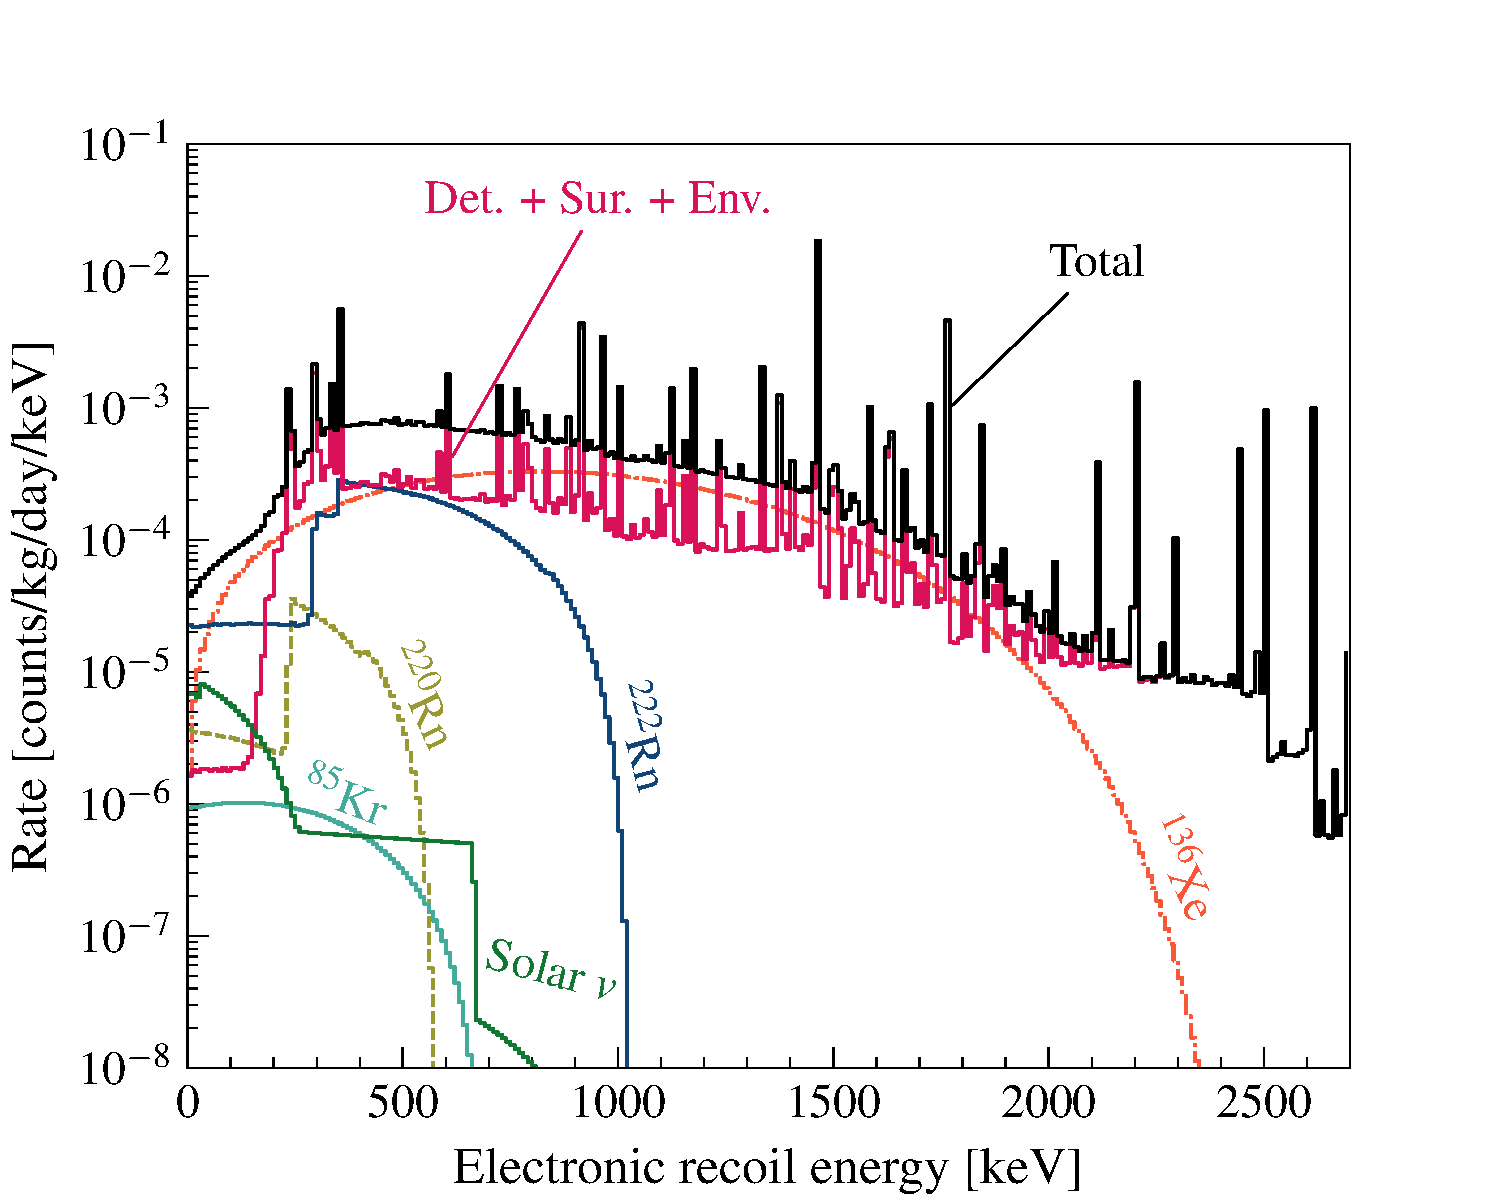
\includegraphics[scale=0.5]{Chapter_5/Figures/er_background_spectrum.pdf}
    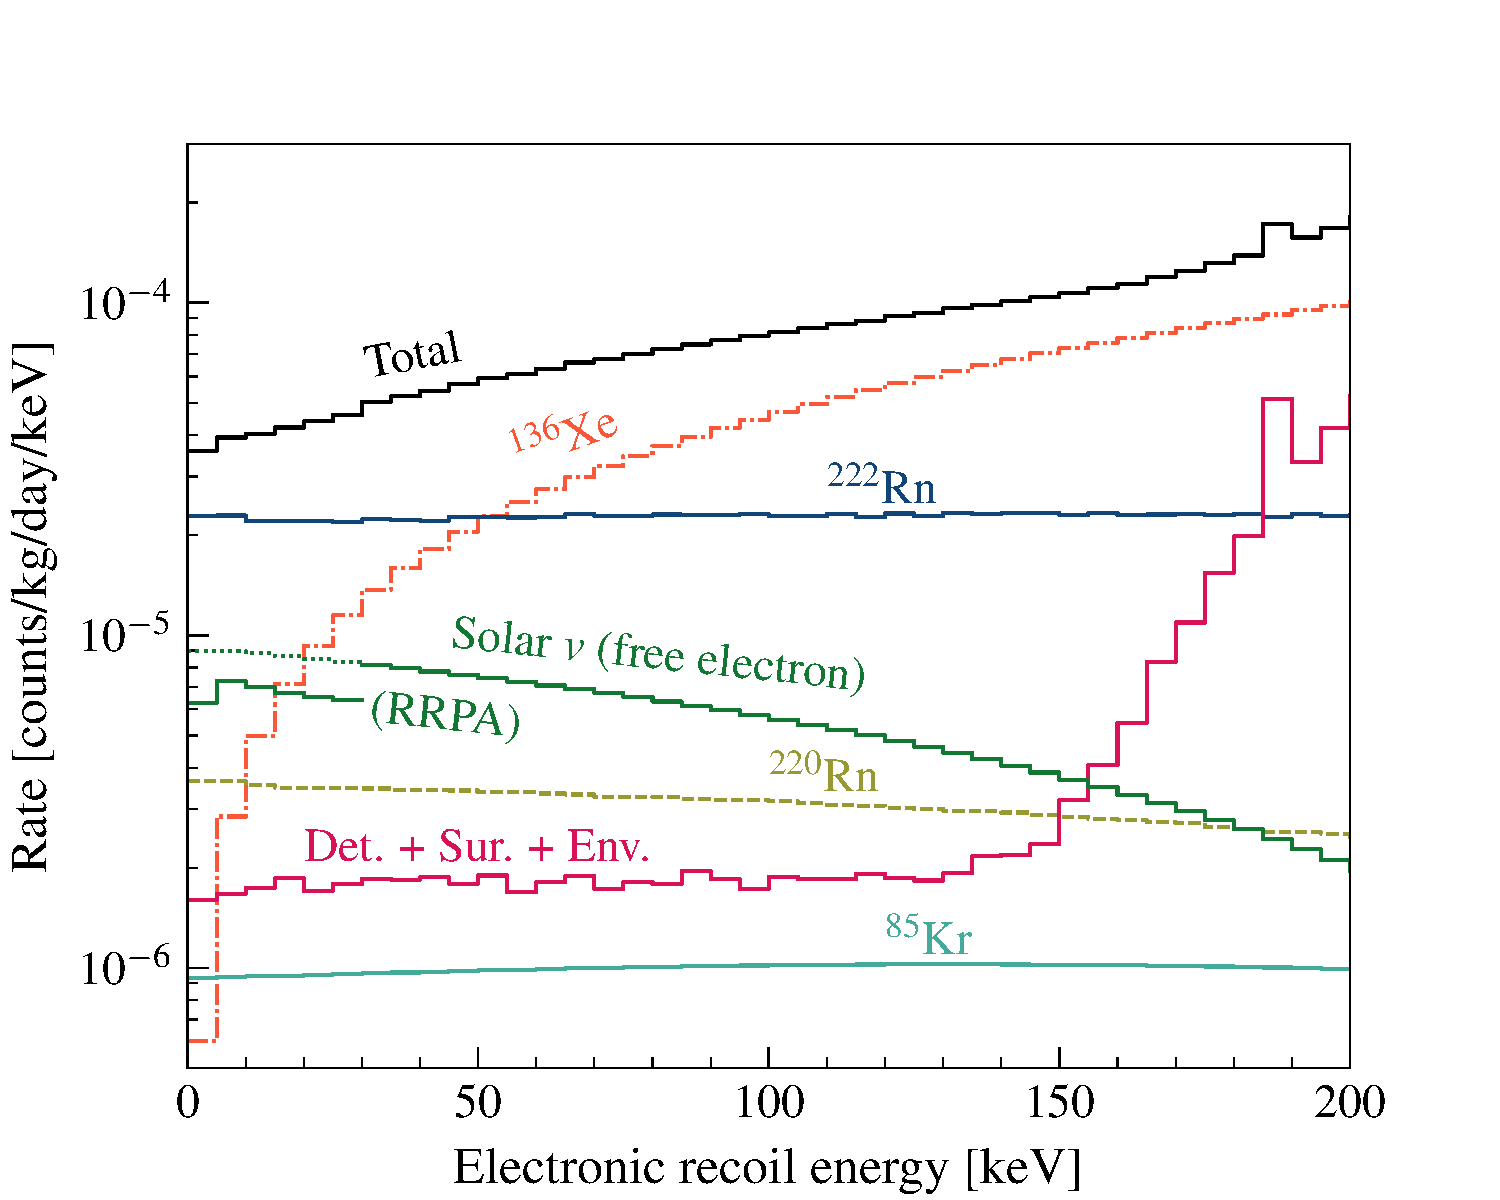
\includegraphics[scale=0.5]{Chapter_5/Figures/er_background_spectrum_zoomed.pdf}
    \caption[The extended (above) and the close-up (below) projections of ER background spectra in the 5.6 tonne fiducial volume for single scatter events, including the skin and OD veto cuts.]%
    {The extended (above) and the close-up (below) projections of ER background spectra in the 5.6 tonne fiducial volume for single scatter events, including the skin and OD veto cuts. Detector efficiency and WIMP-RIO cuts on S1$_{c}$ are also excluded. The scaling applied to the \textit{pp} + \BeS{} + \NOT{} from relativistic random phase approximation (RRPA)calculations is visible below 30 keV \cite{Chen_2017}. Laboratory, cosmogenic and surface backgrounds are combined together as (Det. + Sur. + Env.). Figure adapted from \cite{akerib2018projected}.}
    \label{fig:lz_er_spectrum}
\end{figure}
%


%%------------------------------$$
\section{Statistical Approach}
\label{sec:lz_stats}
%%------------------------------$$

The eventual outcome expected from the LZ experiment is either to discover a dark matter signal that is significantly different from the expected background model---WIMP-like or otherwise, or in a less favourable scenario, verify the expected background model and set a statistical limit on the excluded model parameters. Often the outcome of the experiment is evaluated against the \textit{null} ($H_{0}$) and the \textit{alternative} ($H_{1}$) hypothesis in determining the compatibility of the observed experimental dataset with the hypotheses. In testing for a hypothesis, $H_{0}$ is assumed to be true until it is rejected by the observed dataset. The definition of the null and alternative hypothesis is dependent on the type of statistical statement being made; either claiming a significance for discovery or setting limits on model parameters. 

Typically, new physics searches are looking for a signal that is adding on top of the expected background. The discovery of a signal is formulated by a hypothesis test where the background-only hypothesis plays the role of the null hypothesis and the signal-plus-background hypothesis plays the alternative. In claiming a discovery, the background-only hypothesis is rejected on the bases that it is incompatible with the observed data. When the observed dataset fails to reject the null hypothesis, hence failing to claim a discovery significance, there remains the question of what values of the theoretical parameter space is still allowed---holds potential for discovery, likewise, what values of the model parameter space is excluded with the available data. In the limit setting scenario, the null and the alternative hypothesis are flipped around, where the null hypothesis is defined as the signal-plus-background and the alternative is background-only. Hence, a series of null hypothesis are tested with increasing values of the parameter of interest until a median value is reached for the desired exclusion significance---also known as the confidence region/interval. 

The approach taken in determining the discovery potential and the sensitivity of LZ to WIMPs is the Profile Likelihood Ratio (PLR) method \cite{Rolke_2005} utilising an unbinned maximum likelihood. This method allows an event-by-event comparison of the observed (or pseudo) data to a given model, providing a near-optimal exploration due to its ability to discriminate between signal and background by utilizing a number of variables that may have limited discrimination power on their own. In utilising on this method, a statistical package \textsc{LZStats} was developed that built upon the RooStats package frequently used in the HEP community \cite{moneta2010roostats}. A detailed description of the \textsc{LZStats} package can be found in \cite{ibles}. The following sections will lay out the foundations of the approach taken in \textsc{LZStats}, focusing on the PLR method, construction of the null and the alternative hypothesis for the WIMP search, which become the inputs to \textsc{LZStats} and finally, the output from this package and the construction of the sensitivity and discovery potential of the LZ experiment.


\subsection{Profile Likelihood Ratio Method}
\label{secsec:statistical_terminology}

\subsubsection{Statistical Terminology}

A detector usually records an extensive amount of data of which only a selected few are of interest. The selection criteria for the WIMP search in LZ has been described in section (\ref{secsec:background_selection}). The dataset used in the studies to follow are achieved by Monte Carlo techniques to generate pseudo-experiments under the condition imposed by the hypothesis. Each event is parameterised by a vector $\pmb{x}$ of constructed quantities, known as observables. The observables in LZ data include $S1_{c}$, $S2_{c}$, \textit{x-y-z} and $t$. The spatial quantities are assumed to be uniform due to fiducialisation and events are assumed to be time-independent; hence, these variables are not included in the list of PLR observables. The observables for the WIMP search study are selected as $\pmb{x} = (S1_{c}, \; S2_{c})$, following the definitions of these two quantities from the previous chapter.

The background and signal \textit{event probability models} representing the hypotheses is then constructed as a parametric family of probability density functions (PDF) in obtaining a particular event for a particular background or signal component ($c$) and is expressed by, 
%
\begin{equation}
    f_{c}(\pmb{x}|\pmb{\theta}).
    \label{eq:pdf}
\end{equation}
%
The parameters of the model given by $\pmb{\theta}$ are intrinsic to the model, representing parameters of a physical theory, or an unknown property that can be estimated from data. The complete set of model parameters include the \textit{parameters of interest} (POI), $\pmb{\alpha}$ and the \textit{nuisance parameters}, $\pmb{\nu}$, which account for unknown experimental properties of the physical theory, such as uncertainties; carrying no intrinsic value but necessary for an accurate depiction of the model. The event probability model typically contains a number of background components and a signal component, each with their associated PDFs and an expected mean number of events, $\mu_{c}(\pmb{\theta})$, the sum of which is given by $\mu(\pmb{\theta})$. For a total number of N components, total probability model is then given as the weighted sum of each individual component, where
%
\begin{equation}
    f(\pmb{x}|\pmb{\theta{}}) = \sum_{c=1}^{N}\left(\frac{\mu_{c}(\pmb{\theta})}{\mu(\pmb{\theta})}\right) f_{c}(\pmb{x}|\pmb{\theta}).
    \label{eq:pdf}
\end{equation}
%
In considering a dataset with $n$ events, where $\mathcal{D} = \{\pmb{x}_{i}\}_{i=1}^{n}$ with events as independently drawn from the same underlying distribution, the the \textit{total probability model} takes the form of the product of the individual probability distributions of each event. Furthermore, the overall Poissonian nature of observing $n$ events given $\mu(\pmb{\theta})$ has to be taken into account, resulting in
%
\begin{equation}
    f(\mathcal{D}|\pmb{\theta}) &= Pois(n|\mu(\pmb{\theta}))\prod_{i=1}^{n}f(\pmb{x}_{i}|\pmb{\theta}) \\
    &= \bigg( \frac{\mu(\pmb{\theta})^{n}}{n!}e^{-\mu(\pmb{\theta})} \bigg) \prod_{i=1}^{n}f(\pmb{x}_{i}|\pmb{\theta}).
    \label{eq:pdf}
\end{equation}
%
The final form of the probability density model takes into account the nuisance parameters as approximated Gaussian constraints, which originate from auxiliary measurements. Due to the uncertain nature of these parameters, which contain a degree of uncertainty on the estimate, they are added as a \textit{constraining term}, leading to the fully generalised form of the probability density model
%
\begin{equation}
    f(\mathcal{D}|\pmb{\theta}) &= \MathText{Pois}(n|\mu(\pmb{\theta})) \bigg[ \prod_{i=1}^{n}f(\pmb{x}_{i}|\pmb{\theta}) \bigg] \prod_{j=1}^{N_{c}}g(\pmb{\alpha}_{j}|\nu_{j}),
    \label{eq:final_pdf}
\end{equation}
%
where the constraining term $g(\alpha_{j}|\nu_{j})$ is given as the product of $N_{c}$ constraining functions for each nuisance parameter, $\nu_{j}$.

\subsubsection{Profile Likelihood Ratio}

The likelihood function $\mathcal{L}(\pmb{\theta})$ is numerically equivalent to equation (\ref{eq:final_pdf}) with a fixed $\mathcal{D}$ and is used to determine the combination of model parameter values that maximize the probability of drawing the obtained dataset, $\mathcal{D}_{obs}$. It should be noted that the likelihood function does not represent the probability density for $\pmb{\theta}$ and often does not normalise to unity. The likelihood function is used to investigate the measure of agreement between the observed data and a given hypothesis, through the construction of a function of the measured variables, called a \textit{test statistic} $t(\mathcal{D})$. Although a test statistic can be multidimensional, often it is constructed as a scalar function to lower the dimensionality of the data without losing the ability to discriminate between hypotheses. Each hypothesis will imply a test statistic distribution, i.e. $f(t|H_{0}), \; f(t|H_{1})$; which may be calculated analytically or numerically. Commonly, Monte Carlo techniques are used to generate pseudo-experiments for complicated likelihoods, from which a test statistic distribution is obtained and a statement about the compatibility of the hypotheses is inferred. 

A widely used test statistic for a given parameter of interest $\mu$ and a collection of nuisance parameters $\nu$, is the profile likelihood ratio (PLR) \cite{Rolke_2005, Cowan:2010js}, defined as
%
\begin{equation}
    \lambda(\mu) = \frac{\mathcal{L}(\mu, \pmb{\hat{\hat{\nu}}})}{\mathcal{L}(\hat{\mu}, \pmb{\hat{\nu}})}.
    \label{eq:plr}
\end{equation}
%
The $\pmb{\hat{\hat{\nu}}}}$ represents the value of $\nu$ which maximises the likelihood function for a fixed value of $\mu$, known as the \textit{conditional maximum-likelihood estimator}. The denominator is the maximised (unconditional) likelihood-function estimator of $\mu$, where the single hat refers to the \textit{maximum-likelihood estimators} (MLE), which are defined as the value that which maximises the likelihood function. The impact of the nuisance parameters broaden the profile likelihood as a function of $\mu$, reflecting the lack of information about $\mu$ due to the systematic uncertainties. 

In examining the comparability of hypotheses as a means for limit setting or assessing discovery potentials, it is convenient to use the test statistic
%
\begin{equation}
    t_{\mu} = -2\MathText{log}\lambda(\mu),
    \label{eq:plr_test}
\end{equation}
%
which is distributed between 0 and infinity, with larger values of the test statistic corresponding to increasing incompatibility between the two hypothesis of interest.

\subsubsection{Hypothesis Testing}

Once the distributions of the null and the alternative hypotheses are constructed through the test statistic, it becomes possible to define a hypothesis test to derive a statistical statement on whether the null hypothesis can be rejected. This is achieved through the definition of the \textit{p}-value, defined as the probability of obtaining a result as the observed dataset under the assumption that the null hypothesis $H_{0}$ is true, i.e.
%
\begin{equation}
    p &= P(t>t_{obs}|H_{0}), \\
    &= \int_{t_{obs}}^{\infty} f(t|H_{0})dt.
    \label{eq:p_value}
\end{equation}
%
A hypothesis test is constructed where a critical region is defined with a pre-declared size $\alpha$ such that the null hypothesis $H_{0}$ is rejected if the observed test statistic $t_{obs}$ falls in this region, i.e. $p < \alpha$. The confidence level (CL) of the test is defined as ($1-\alpha$)\%, where the size of $\alpha$ is typically given as 5\% or 10\%. In direct detection of dark matter and in this work, the CL is set to 90\%. In particle physics, a common practice of reporting statistical results of a hypothesis test is via the significance Z, given as
%
\begin{equation}
    Z = \Phi^{-1}(1-p),
    \label{eq:significance}
\end{equation}
%
where $\Phi^{-1}$ is the inverse of the cumulative distribution of a standard Gaussian. Z represents the number of standard deviations above the mean of a normal Gaussian distribution such that the upper-tail probability is equal to the \textit{p}-value. The significance for evidence or a discovery correspond to $5\sigma > Z	 \geq 3\sigma$ and $ \geq 5\sigma$, respectively.


\subsection{Input}
\label{secsec:plr_input}

The background only hypothesis for the PLR analysis is constructed by an 11-component background model that is based on the analysis selection criteria detailed in section (\ref{secsec:background_selection}). The estimated number of counts per component in the extended $S1_{c}\mhyphen{}S2_{c}$ space and their corresponding uncertainties that feed into the PLR analysis as the nuisance parameter terms is shown in table (\ref{tab:lz_pdf_estimations}). The component specific uncertainties are estimated on a component-by-component basis. The \textit{Det. + Sur. + Env.} uncertainties for both ER and NR contributions come from counting and simulation results, those on the neutrino components are primarily flux uncertainties, and the uncertainties on radon are from the branching ratio uncertainty of \PbTOF{} and \PbTOT{} to their respective ground states. Finally, those on \KrEF{} and \XeOTS{} are estimates from uncertainties on the spectral shapes at low energies. Although these systematics are treated as nuisance terms in the LZ PLR with Gaussian priors, preliminary studies on their significance result in minimal shifts in the sensitivity results due to the low number of background counts expected in LZ. No other nuisance terms are included in the sensitivity calculation presented here. 

%
\begin{table}[t!]
\centering
\caption
[Eleven background types considered in the PLR analysis, along with the integrated counts in the LZ 1000 day WIMP search exposure and the systematic uncertainties on their normalisations, included as nuisance parameters in the PLR.]
{Eleven background types considered in the PLR analysis, along with the integrated counts in the LZ 1000 day WIMP search exposure and the systematic uncertainties on their normalisations, included as nuisance parameters in the PLR. Counts are for the WIMP search ROI (S1 with $\geq$ 3−fold coincidence, S1c < 80 phd and uncorrected S2 > 415 phd): approximately 1.5–15 keV for ERs and 4–60 keV for NRs; and after application of the single scatter, skin and OD veto, and 5.6 tonne fiducial volume cuts.}
\label{tab:lz_pdf_estimations}
\vspace{1mm}
\renewcommand{\arraystretch}{1.2}
    \begin{tabularx}{0.9\linewidth}{@{\extracolsep{\fill}}llll}
    \toprule
    \textbf{Background Components} & %1
    \textbf{} & %2
    \textbf{Counts (N)} & %3
    \textbf{Uncertainty ($\sigma/N$)} & %3
    \hline
    \hline
    \textbf{ER}    &      &      \\
    Det. + Sur. + Env. & $\mu_{DetER}$ & 152 & 20\% \\
    \RnTTT{} & $\mu_{Rn\MathText{-}222}$ & 1705 & 10\% \\
    \RnTTZ{} & $\mu_{Rn\MathText{-}220}$ & 281 & 10\% \\
    \XeOTS{} \twoNeutrinoDoubleBeta{} & $\mu_{vvBB}$ & 406 & 50\% \\
    \KrEF{} & $\mu_{Kr\MathText{-}85}$ & 74 & 20\% \\
    Solar $\nu$ (\textit{pp} + \BeS{} + \NOT{}) & $\mu_{pp}$ & 548 & 2\% \\
    \textbf{NR}    &      &      \\
    Det. + Sur. + Env. & $\mu_{DetNR}$ & 0.77 & 20\% \\
    Atmospheric $\nu$ (Atm)  & $\mu_{atm}$ & 0.64 & 25\% \\
    Diffuse supernova $\nu$ (DSN) & $\mu_{DSN}$ & 0.14 & 50\% \\
    \textit{hep} $\nu$ & $\mu_{hep}$ & 0.78 & 15\% \\
    \BE{} $\nu$ & $\mu_{B\MathText{-}8}$ & 29 & 4\% \\
    
    \bottomrule
    \end{tabularx}
\end{table}
%

The background-only event probability model for the WIMP search is constructed from the expected spectral background as given in figures (\ref{fig:lz_nr_spectrum} \& \ref{fig:lz_er_spectrum}), where component specific PDFs in the $S1_{c}\mhyphen{}S2_{c}$ space, normalised to the background specific expected number of events is shown in figure (\ref{fig:lz_background_pdfs}). The background PDFs, $f_{b}(\pmb{x_{i}}})$, include no implicit dependence on any model parameters, i.e., no shape-varying nuisance parameters such as $g_1$ or $g_2$. These distributions are generated by taking samples from the corresponding recoil energy spectra and converting them into the corrected (flat-fielded) S1 and S2 signals with the application of LZ specific detector parameters as detailed in section (\ref{secsec:detector_param}), by using NEST. As previously mentioned, the PLR analysis does not take into account any position related information, as majority of the background sources are expected to be uniformly distributed. The non-uniformity observed closer to the TPC walls, arising from detector the \textit{Det. + Sur. + Env.} component is largely minimised due to fiducialisation.

The full LZ likelihood function for the WIMP search includes the signal spectrum for the WIMP recoils at varying WIMP mass, $m_{\chi}$. The signal spectra are calculated using the standard halo model as discussed in detail in section (\ref{subsec:wimp_dm}) with $v_{0} = 220 \; \MathText{km/s}$, $v_{esc} = 544 \; \MathText{km/s}$ and $\rho_{0} = 0.3 \; \MathText{GeV/c}^2$. The SI WIMP-nucleon recoil rate is calculated using the Helm from factor, as provided in \cite{PhysRev.104.1466}, whereas the SD WIMP-nucleon recoil rate is driven from nuclear structure functions from \cite{PhysRevD.88.083516}. The full sensitivity is calculated over a range of WIMP mass, $m_{\chi}$, where a PDF for each mass is used as a standalone signal hypothesis to be tested. The power of the PLR technique arises from an optimal weighting of the background-free and background-rich regions, and for all WIMP masses considered background rejection exceeds 99.5\% for a signal acceptance of 50\%. An example pseudo-experiment simulated from the total probability model in the $S1_{c}\mhyphen{}S2_{c}$ space as expected by the LZ experiment after the completion of a full 1000 live-day run is shown in figure (\ref{fig:lz_1000_day_run}). 

The simulated dataset in figure (\ref{fig:lz_1000_day_run}) corresponds to a background-only scenario in which majority of the events will occur in the ER band of the $S1_{c}\mhyphen{}S2_{c}$ space. The ER and NR bands discussed previously in section (\ref{subsubsec:recom_disc} in highlighting the discrimination power between the two event types are shown here in blue and red, respectively. Furthermore, backgrounds expected from \BE{} + \textit{hep} neutrinos and a potential 40 GeV/c\squared{} signal as seen in the $S1_{c}\mhyphen{}S2_{c}$ space is overlaid with their corresponding $1\sigma$ and $2\sigma$ contours. The signal contour is a direct consequence of the standard halo model of WIMPs. In setting limits, studying the sensitivity or the discovery potential of the detector, the parameter of interest is represented by the signal mean $\mu_{s}(\sigma)$ of a specific WIMP mass, which is directly proportional to the WIMP-nucleon scattering cross-section. Moreover, the expected mean of each background component $\mu_{b}$ assumes a degree of uncertainty as specified in table (\ref{tab:lz_pdf_estimations}), thus is varied in the PLR analysis with a Gaussian variability constraint. The full log-likelihood function utilised by LZ for the WIMP analysis is thus given by the equation:

%
\begin{equation}
    \begin{split}
    - 2\MathText{log}\mathcal{L}(\mu_{s}(\sigma), \pmb{\nu}) = \; &2\left(\mu_{s} + \sum_{b=1}^{N_{c}}\mu_{b} \right) \\
    &- 2\sum_{i=1}^{n_{0}} \MathText{log} \left( \mu_{s}(\sigma)f_s(\pmb{x}_{i}|m_{\chi})
    + \sum_{b=1}^{N_{c}} \mu_{b}f_{b}(\pmb{x}_{i}) \right) \\
    &+ \sum_{b=1}^{N_{c}} \frac{(\mu_{b}-n_{b})^{2}}{\nu_{b}^{2}},
    \end{split}
    \label{eq:full_lz_likelihood}
\end{equation}
%
where $\pmb{\nu}$ represents the set of all nuisance parameters, $n_{b}$ and $\nu_{b}$ refer to the estimated number of counts of a given background component in the WIMP search ROI and its associated uncertainty, respectively. The subscript i runs over each of the $n_{0}$ events in the dataset and b runs over each background component; evaluating the full LZ WIMP likelihood.  

\begin{figure}[h!]
    \centering
    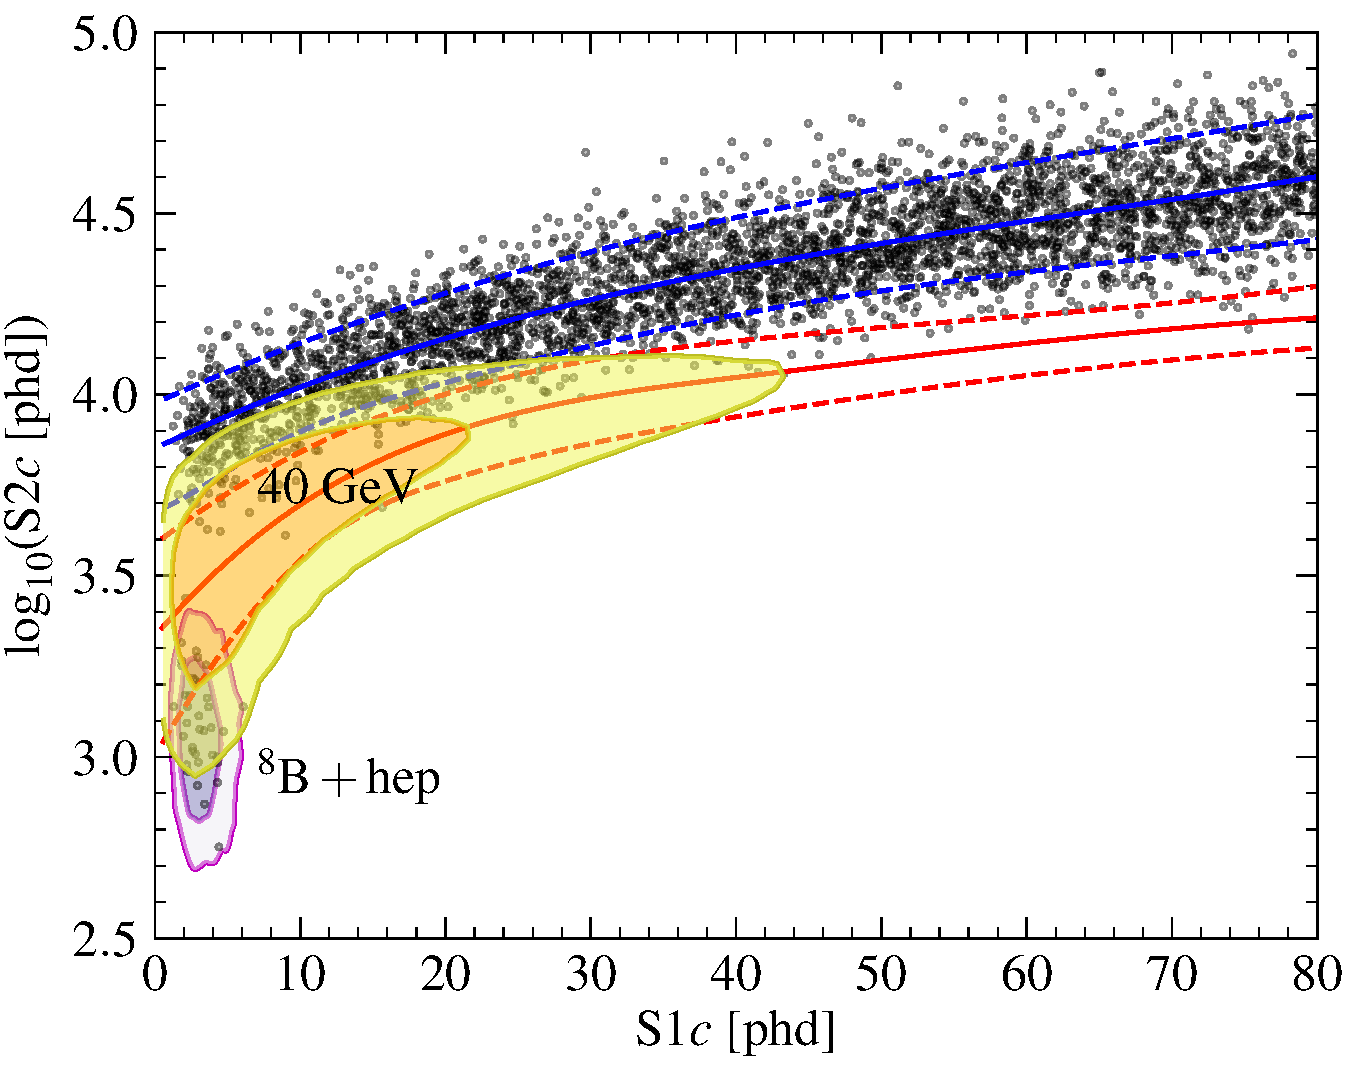
\includegraphics[scale=0.6]{Chapter_5/Figures/sensitivity_studies/background_with_40_gev_wimp.pdf}
    \caption[LZ simulated data set for a background-only 1000 live day run and a 5.6 tonne fiducial mass. ER and NR bands are indicated in blue and red, respectively (solid: mean; dashed: 10\% and 90\%). The $1\sigma$ and $2\sigma$ contours for the low-energy \BE{} and \textit{hep} NR backgrounds, and a 40 GeV/c\squared{} WIMP are shown as shaded regions.]%
    {LZ simulated data set for a background-only 1000 live day run and a 5.6 tonne fiducial mass. ER and NR bands are indicated in blue and red, respectively (solid: mean; dashed: 10\% and 90\%). The $1\sigma$ and $2\sigma$ contours for the low-energy \BE{} and \textit{hep} NR backgrounds, and a 40 GeV/c\squared{} WIMP are shown as shaded regions.}
    \label{fig:lz_1000_day_run}
\end{figure}
%

%
\begin{figure}[h!]
    \centering
    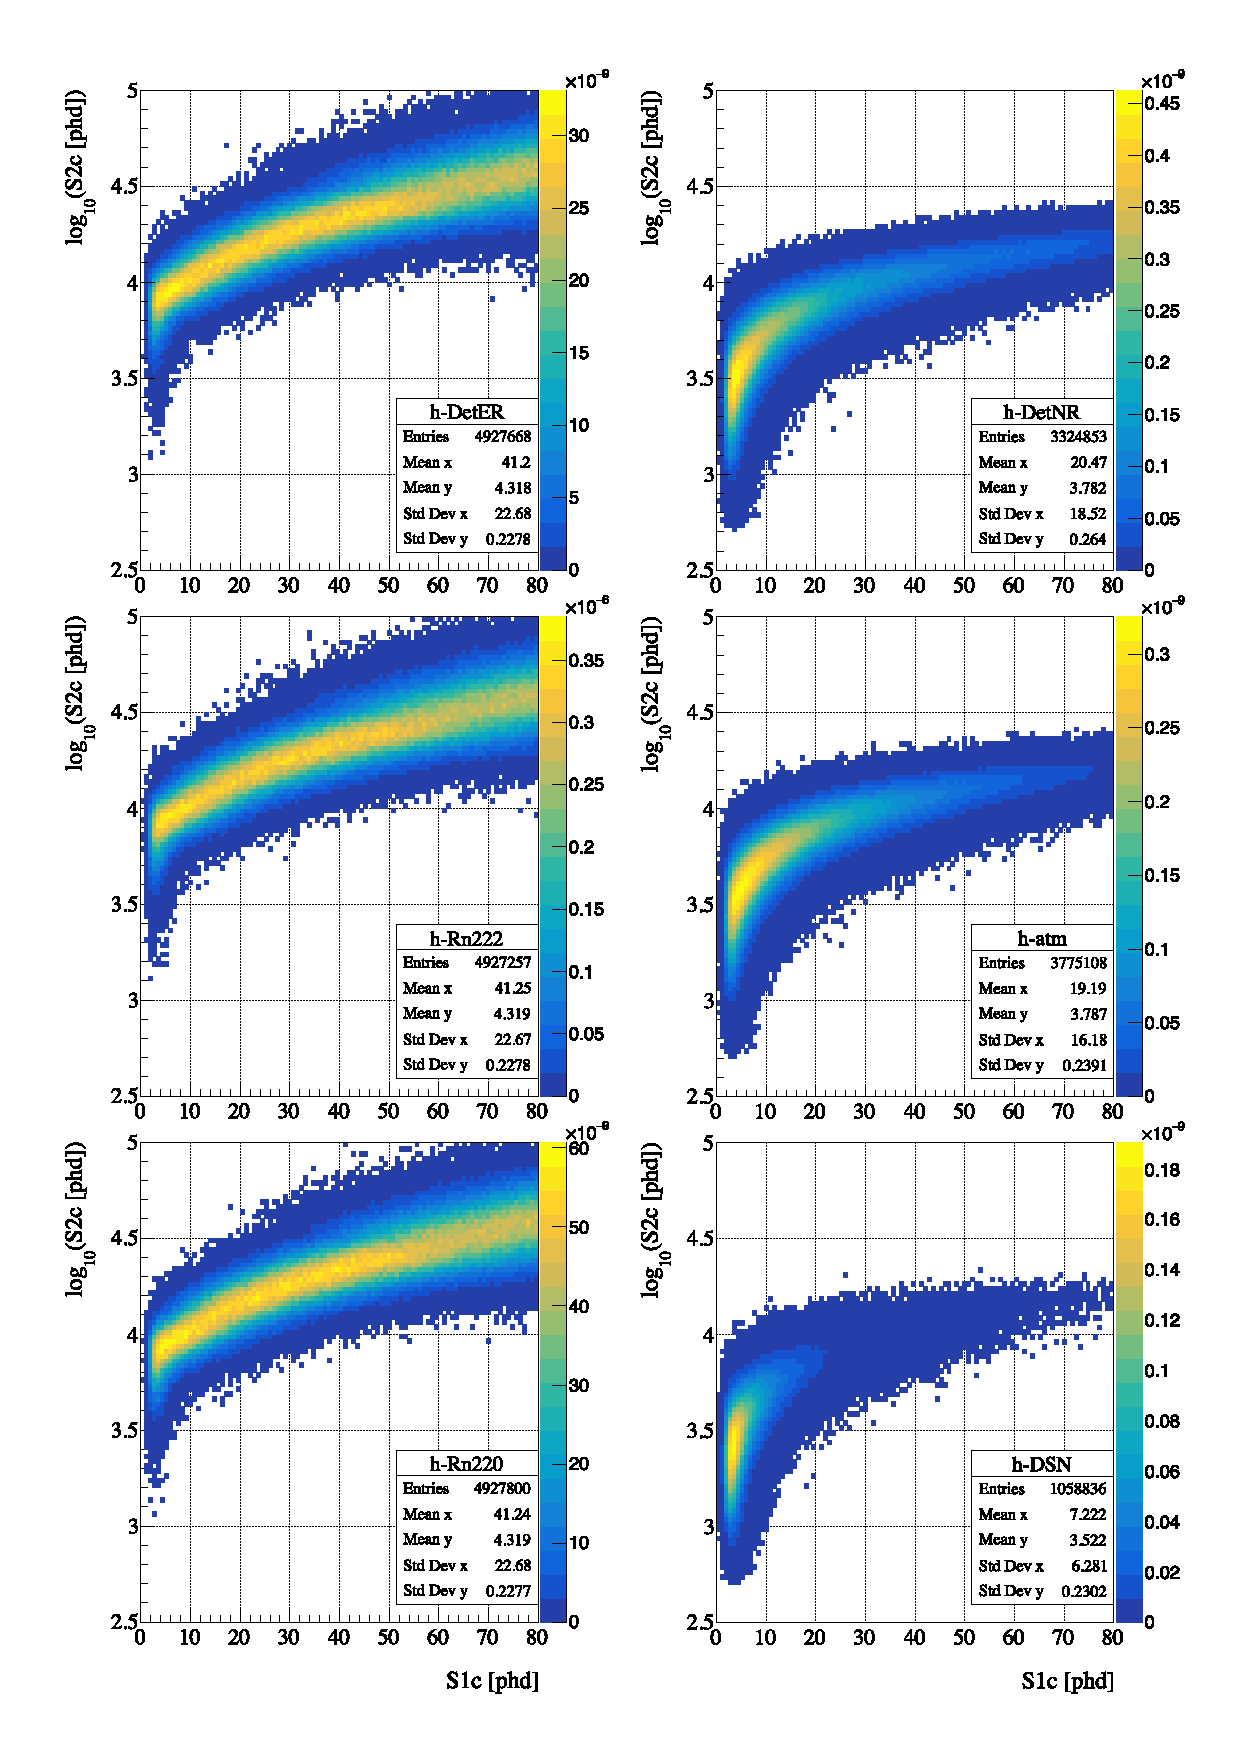
\includegraphics[scale=0.7]{Chapter_5/Figures/sensitivity_studies/background_pdfs_1.pdf}
    \caption[Background components of the event probability model for the WIMP search ROI with the electronic recoil background PDFs (left) and nuclear recoil background PDFs (right) normalised to their specific contribution in the corrected $S1\mhyphen{}S2$ space.]%
    {Background components of the event probability model for the WIMP search ROI with the electronic recoil background PDFs (left) and nuclear recoil background PDFs (right) normalised to their specific contribution in the corrected $S1\mhyphen{}S2$ space.}
    \label{fig:lz_background_pdfs}
\end{figure}
%
\begin{figure}[h!]
    \ContinuedFloat 
    \centering
    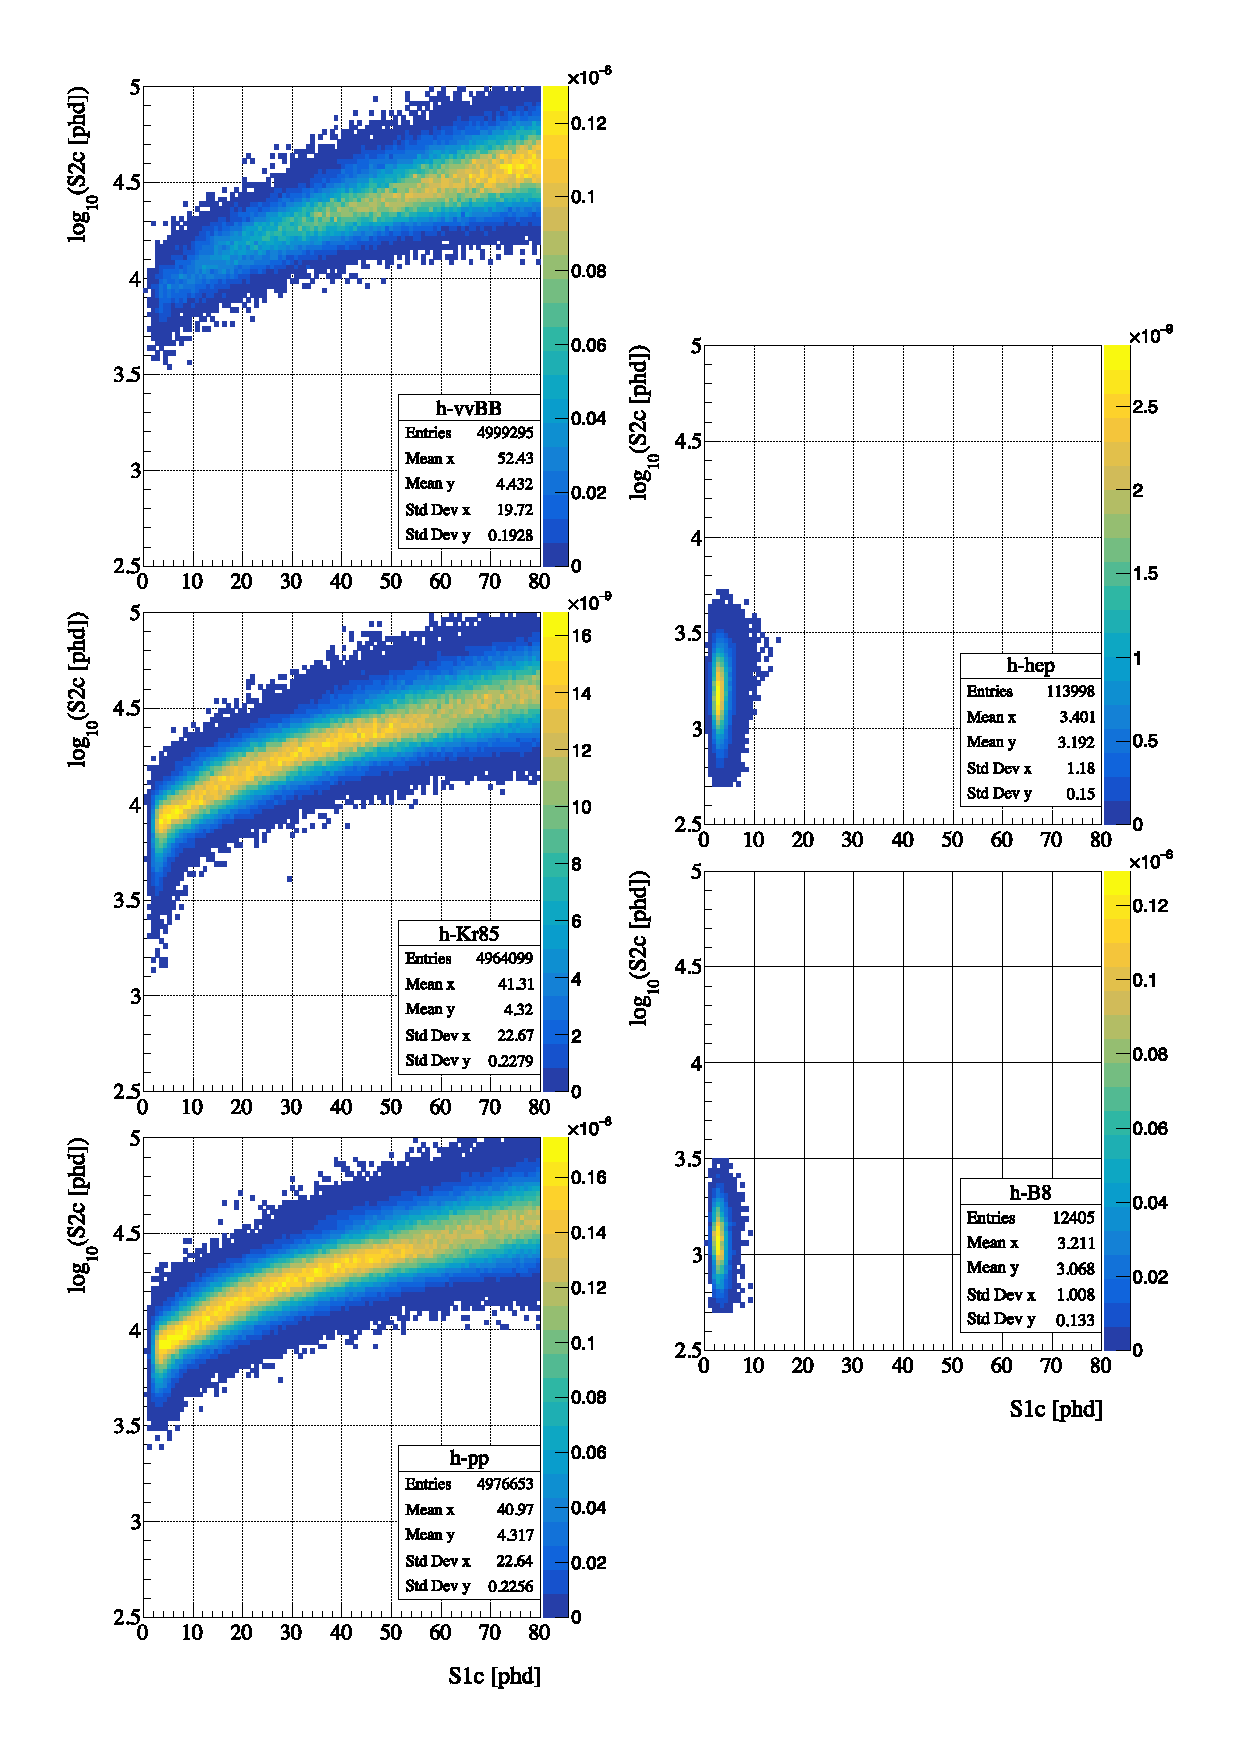
\includegraphics[scale=0.7]{Chapter_5/Figures/sensitivity_studies/background_pdfs_2.pdf}
    \caption[Background components of the event probability model for the WIMP search ROI with the electronic recoil background PDFs (left) and nuclear recoil background PDFs (right) normalised to their specific contribution in the corrected $S1\mhyphen{}S2$ space.]%
    {Background components of the event probability model for the WIMP search ROI with the electronic recoil background PDFs (left) and nuclear recoil background PDFs (right) normalised to their specific contribution in the corrected $S1\mhyphen{}S2$ space.}
    \label{fig:lz_background_pdfs}
\end{figure}
%

\clearpage

\subsection{Output}
\label{secsec:detector_param}

The statistical statement inferred by setting a limit or a sensitivity curve in the case of an experimental projection prior to data taking, is one which tries to determine the amount of a potential signal that can be present until the null hypothesis is no longer justifiable to a certain confidence level. Hence, the goal is to find the value of the POI, in this case, the number of detected WIMP particle interactions above which the signal plus background ($S+B$) hypothesis is incompatible with the background-only ($B_{only$) hypothesis at a 90\% CL. Therefore, the signal strength $\mu_{s}$ is scanned over to construct a multitude of test statistic distributions to determine the value of $\mu_{s}$ at which the statistical statement is achieved. 

The corresponding one-sided PLR test statistic distributions from a 40 GeV/c\squared{} SI-WIMP interaction is shown in the upper panel of figure (\ref{fig:plr_hypothesis_distributions}) for 16 values of the PIO where $\mu_{s}$ is scanned from 0--16. The null distribution corresponding to the $S+B$ hypothesis of an increasing $\mu_{s}$ is shown from top left to bottom right. The median of the alternative hypothesis representing the $B_{only}$ scenario is taken as a proxy for the observed test statistic (vertical black line). The median alternative hypothesis test statistic used for a projected limit would otherwise be substituted for the observed dataset in the presence of real data. The lower panel in figure (\ref{fig:plr_hypothesis_distributions} represents the \textit{p}-values (black dots) calculated from the pseudo experiments generated through the use of a Monte Carlo method of the above panel. A \textit{p}-value is obtained for each hypothesis test, which represents the value of $\mu_{s}$ used in constructing the $S+B$ hypothesis. Moreover, for each value of $\mu_{s}$ that is tested, $1\sigma$ and $2\sigma$ deviations from the median of the alternative hypothesis is also obtained, represented in green and yellow, respectively. These are representative of the possible statistical and systematic fluctuations of the observed upper limit over repeated experiments.

\begin{figure}[H!]
    \centering
    \vspace{-1cm}
    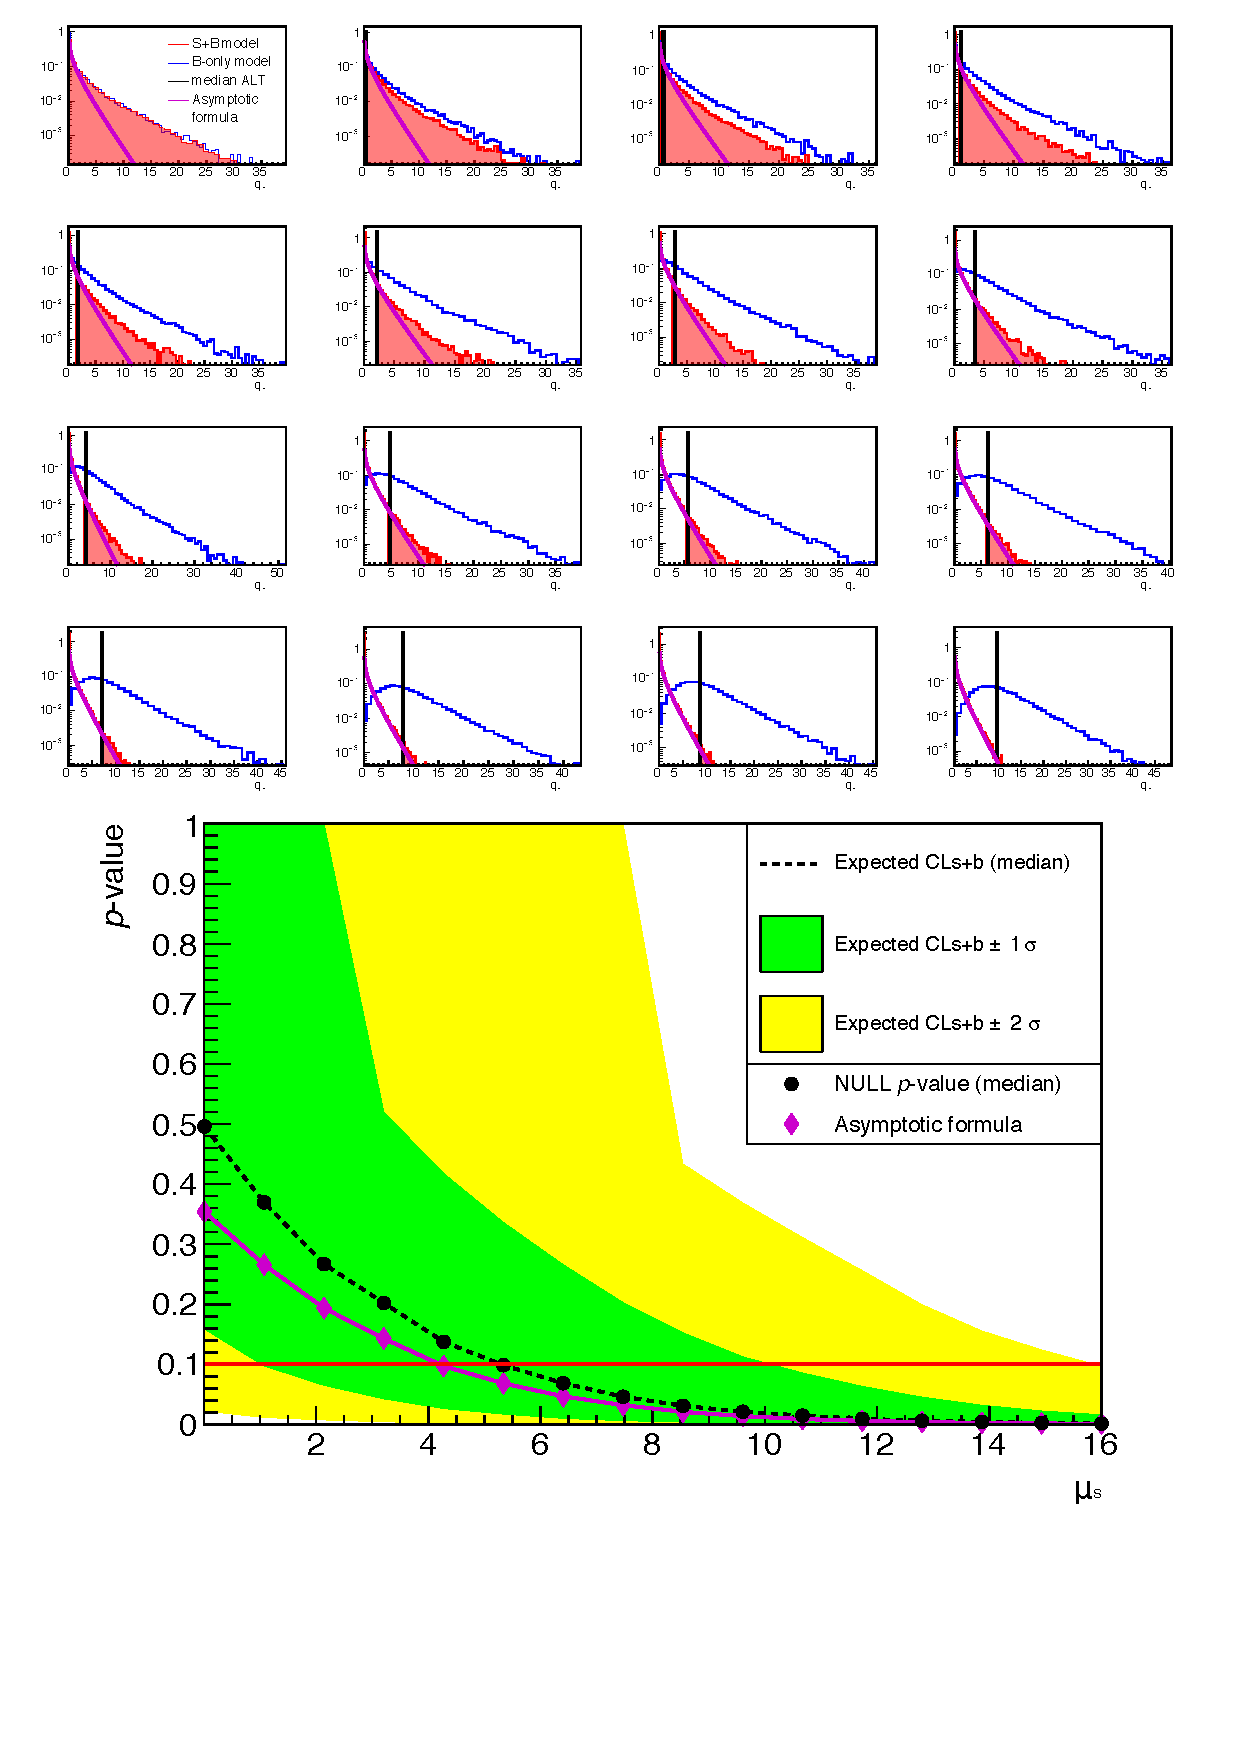
\includegraphics[scale=0.72]{Chapter_5/Figures/sensitivity_studies/statistical_distributions.pdf}
    \caption[The projected sensitivity output from the \textsc{LZStats} package used for the PLR analysis. The plot above shows all of the test statistic distributions under the null and the alternative hypothesis and the plot below shows the null \textit{p}-value calculated from the Monte Carlo and the asymptotic formula.]%
    {The projected sensitivity output of a 40 GeV/c\squared{} WIMP as analysed through the PLR analysis using \textsc{LZStats}. \textit{Above}: Shows the test statistic distributions under the null (signal plus background in red) and the alternative (background-only in blue), constructed using the one-sided PLR test statistic in equation (\ref{eq:plr_test}). The vertical black line indicates the median of the alternative distribution used in calculating the median \textit{p}-value of the hypotheses. Increasing values of the POI, $\mu_{s}$ is tested from top left to bottom right. \textit{Below}: Shows the calculated null \textit{p}-value from both Monte Carlo (black dots) and the asymptotic formula (magenta diamonds). The \textit{p}-value assuming $1\sigma$ and $2\sigma$ shifts from the median of the alternative distribution for each hypothesised $\mu_{s}$ are also indicated with green and yellow bands, respectively. The 90\% upper limit on the POI is obtained when the two hypotheses result in a disagreement where the median \textit{p}-value is equal to or less than 0.1; represented by the horizontal red line.}
    \label{fig:plr_hypothesis_distributions}
\end{figure}
%

The projected 90\% CL upper limit on the POI, $\mu_{s}^{90\%}$, is obtained by determining the point at which the two hypotheses are no longer in agreement with one another; when the agreement between the two hypotheses fall to 10\%. This is indicated as the point at which the \textit{p}-value of a given $\mu_{s}$ is equal to 0.1, as shown by the horizontal red line in figure (\ref{fig:plr_hypothesis_distributions}). 

An alternative statistical test is to determine the projected discovery significance of an input signal model. In this case, the null hypothesis in the limit setting scenario is replaced by the background-only hypothesis and similarly, increasing values of the POI are considered. The projected discovery significance at a $3\sigma$ level is calculated by using the median of the $S+B$ alternative hypothesis until a \textit{p}-value of 0.14\% is reached, where
%
\begin{equation}
    \begin{split}
    p(\mu_{s}^{3\sigma}) &= 1 - \Phi(3) \\
    &= 0.0014. 
    \end{split}
    \label{eq:full_lz_likelihood}
\end{equation}
%
The $\Phi(Z)$ in the above equation is the normal cumulative function. In addition, an alternative method in calculating sensitivity and discovery potential to that of the frequentest method using the asymptotic formula is represented by the magenta lines in figure (\ref{fig:plr_hypothesis_distributions}. This alternative way is not the focus of this thesis, but more information on this can be found in \cite{ibles}. The final sensitivity and discovery potential curves for the LZ experiment are computes across a range of WIMP masses using the statistical methodology described in this section. The following sections will highlight several of these studies, conducted due to the uncertainties arising as a result of the construction phase of the experiment. These are followed by the final projections of the LZ experiment to galactic WIMP dark matter.


%%------------------------------$$
\section{Impact of Radon on Sensitivity and Discovery Potential}
\label{sec:radon_impact}
%%------------------------------$$

The simplified cut-and-count analyses detailed in section (\ref{secsec:background_table}) resulted in a total of 1131 ER and 1.03 NR background events over the duration of a 1000 live day experiment in the WIMP region of interest. A significant proportion of these events are as a result of radon emanation from detector material. In assuming a \RnTTT{}(\RnTTZ{}) activity of 1.81(0.09) \micro{}Bq/kg within the LXe active volume, the approximated events arising from these two sources add up to 792 ER interactions, making up $\sim70\%$ of all ER events, as summarised in table (\ref{tab:lz_background_count}). However, as discussed in detail in section (\ref{sec:lzradon}), the radon emanation projections arising from both the bottom-up and large scale screening efforts of detector materials in LZ come with a range of possible activities. These depend on the performance of the radon removal system in gas, the uncertainties of cold temperature suppression across different material and any systematics that may otherwise be unaccounted. Moreover, the unexpected radon emanation rate observed from the titanium cryostat risked the possibility of failing to reach the sensitivity requirement of $3.0 \times 10^{-48} \; \MathText{cm}^2$ for the SI-WIMP hypothesis as defined by the LZ technical design report \cite{lz_tdr}. 

In order to address these range of possibilities, the potential impact of unexpected radon emanation rates were examined for a range of radon activities, assessing the variability of sensitivity and discovery potential to the SI-WIMP hypothesis. The uniformity of the \RnTTT{} background in the fiducial volume lead to the realisation of an invariable spectral shape under a varying normalisation factor to the radon background. Therefore, a linear shift in normalisation---or the expected activity of radon---results in a vertical spectral shift of the \RnTTT{} and \RnTTZ{} rates provided in figure (\ref{fig:lz_er_spectrum}). By utilising on this idea, the \textsc{LZStats} framework was used to alter the levels of expected radon emanation of the background model, $\mu_{^{222}Rn}$, ranging from 0.1 \micro{}Bq/kg to 10.0 \micro{}Bq/kg of radon activity. Although the results are given in \RnTTT{} specific activity, the \RnTTZ{} activity was also scaled by the same factor, keeping the ratio of \RnTTT{}/\RnTTZ{} constant at all times. 

To accurately explore the potential impact of radon, roughly $200$k pseudo-experiments were produced for each new background hypothesis driven from $\mu_{^{222}Rn}$ and repeated over 16 test values of the POI ($\mu_{s}$) to calculate the \textit{p}-value of the corresponding one-sided median 90\% CL. The change in SI-WIMP sensitivity of a 40 GeV/c\squared{} WIMP as a function of \RnTTT{} activity and the corresponding $3\sigma$ discovery potential is shown in figure (\ref{fig:radon_vs_sensitivity}). These plots are overlaid with the best and the worst possible expected radon emanation scenarios driven from section (\ref{sec:lzradon}); where scenario A (11.0 mBq) represents a rate assuming radon removal (RR) in gas and optimistic cold suppression (CS) factors; B (21.6 mBq) assumes RR and moderate CS factors. Scenarios C (41.3 mBq) and D (60.8 mBq) represent RR-only and warm emanation results, respectively, where CS is not assumed. The projected radon emanation rate given by the vertically dashed green line as assumed in \cite{akerib2018projected} is given as 1.81 \micro{}Bq/kg, situated between scenarios A and B. As observed from figure (\ref{fig:lz_er_spectrum}), both the sensitivity and the discovery potential gradually increases with an increasing radon activity. However, this increase is substantially slow over the range of possible radon scenarios, with the median 90\% CL limit staying well below the LZ requirement of $3.0 \times 10^{-48} \; \MathText{cm}^2$. 

%
\begin{figure}[H!]
    \centering
    \vspace{-1cm}
    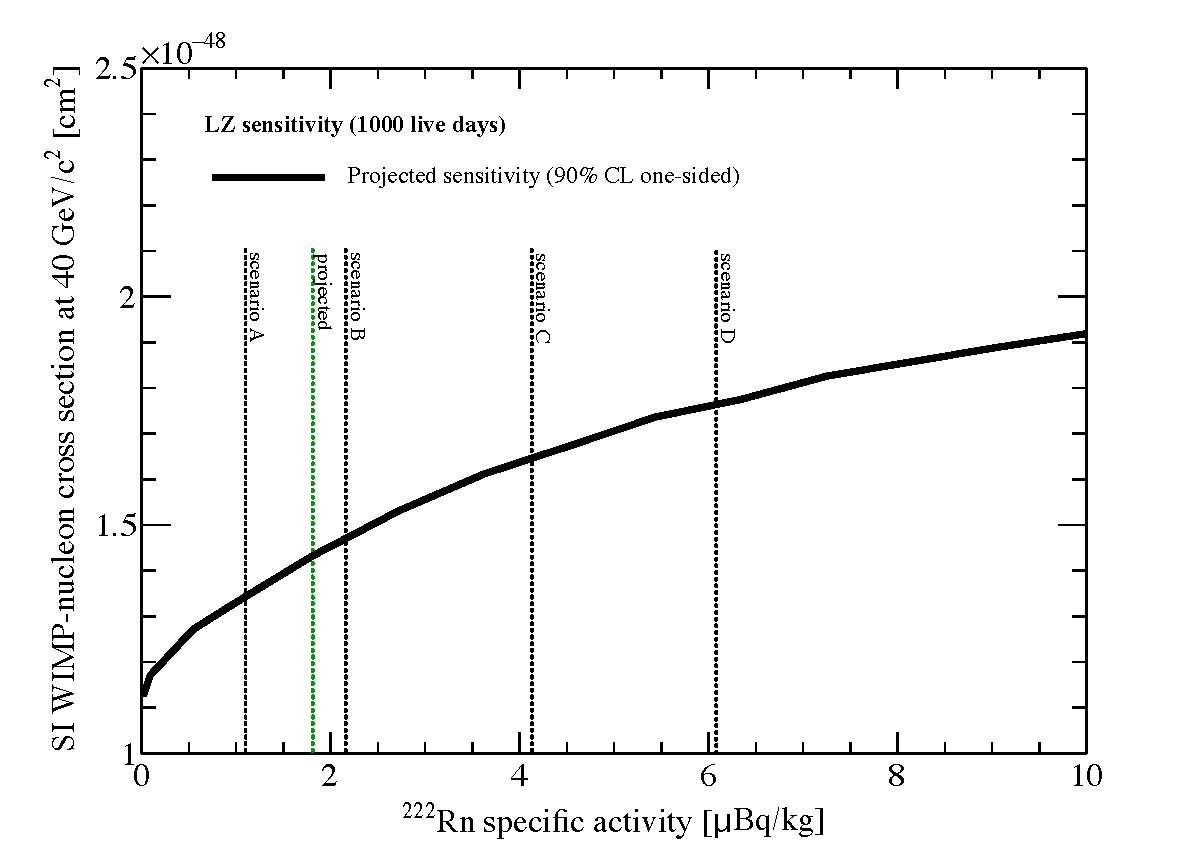
\includegraphics[scale=0.68]{Chapter_5/Figures/sensitivity_studies/radon_sensitivity.pdf}
    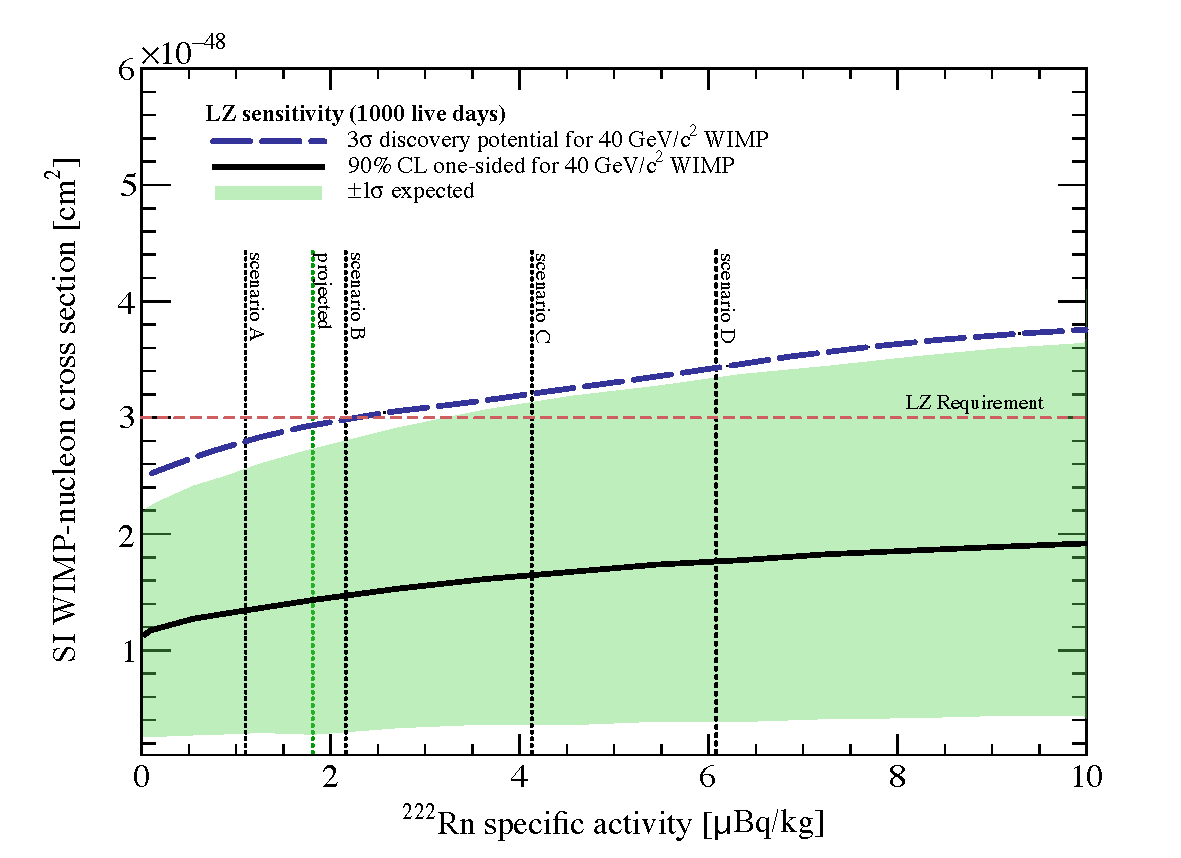
\includegraphics[scale=0.68]{Chapter_5/Figures/sensitivity_studies/radon_sensitivity_discovery.pdf}
    \caption[Projected SI sensitivity and discovery potential for a 1000 live-days run in 5.6 tonnes of fiducial volume as a function of \RnTTT{} activity as observed in the fiducial volume for a WIMP mass of 40 GeV/c\squared{} WIMP.]%
    {Projected SI sensitivity and discovery potential for a 1000 live-days run in 5.6 tonnes of fiducial volume as a function of \RnTTT{} activity as observed in the fiducial volume for a WIMP mass of 40 GeV/c\squared{} WIMP. \textit{Above}: Shows the median 90\% CL sensitivity with the projected estimate for \RnTTT{} activity of 1.81 \micro{}Bq/kg marked with a green vertical line. Scenarios A, B, C and D (black vertical lines) are driven from emanation results in section (\ref{sec:lzradon}), indicating the four scenarios ranging from the most optimistic to the pessimistic scenarios. \textit{Below}: Shows the same result as above but with the variation observed on the $1\sigma$ band of the median sensitivity and the $3\sigma$ discovery potential as radon activity is increased. The LZ sensitivity requirement of $3.0 \times 10^{-48} \; \MathText{cm}^2$ is given with the horizontally dashed red line.}
    \label{fig:radon_vs_sensitivity}
\end{figure}
%

At a \RnTTT{} activity of 1.81 \micro{}Bq/kg, the achieved sensitivity is $1.43 \times 10^{-48} \; \MathText{cm}^2$; whereas with the best (A) and worst (D) possible scenarios, the sensitivity shifts from $1.34 \times 10^{-48} \; \MathText{cm}^2$ to $1.76 \times 10^{-48} \; \MathText{cm}^2$. A drastic increase of 3.4 times (scenario D) in comparison to the baseline radon projection seems to result in a subtle loss is sensitivity, this loss is equivalent to $\sim23\%$ of the baseline sensitivity. To further examine the impact of elevated radon activity within the active volume, statistical tests were conducted to quantify the time impact of such elevated rates; i.e., given an increase of a factor $x$, how much longer does the experiment have to run to reach the desired sensitivity under the baseline projection scenario. 

%
\begin{figure}[H!]
    \centering
    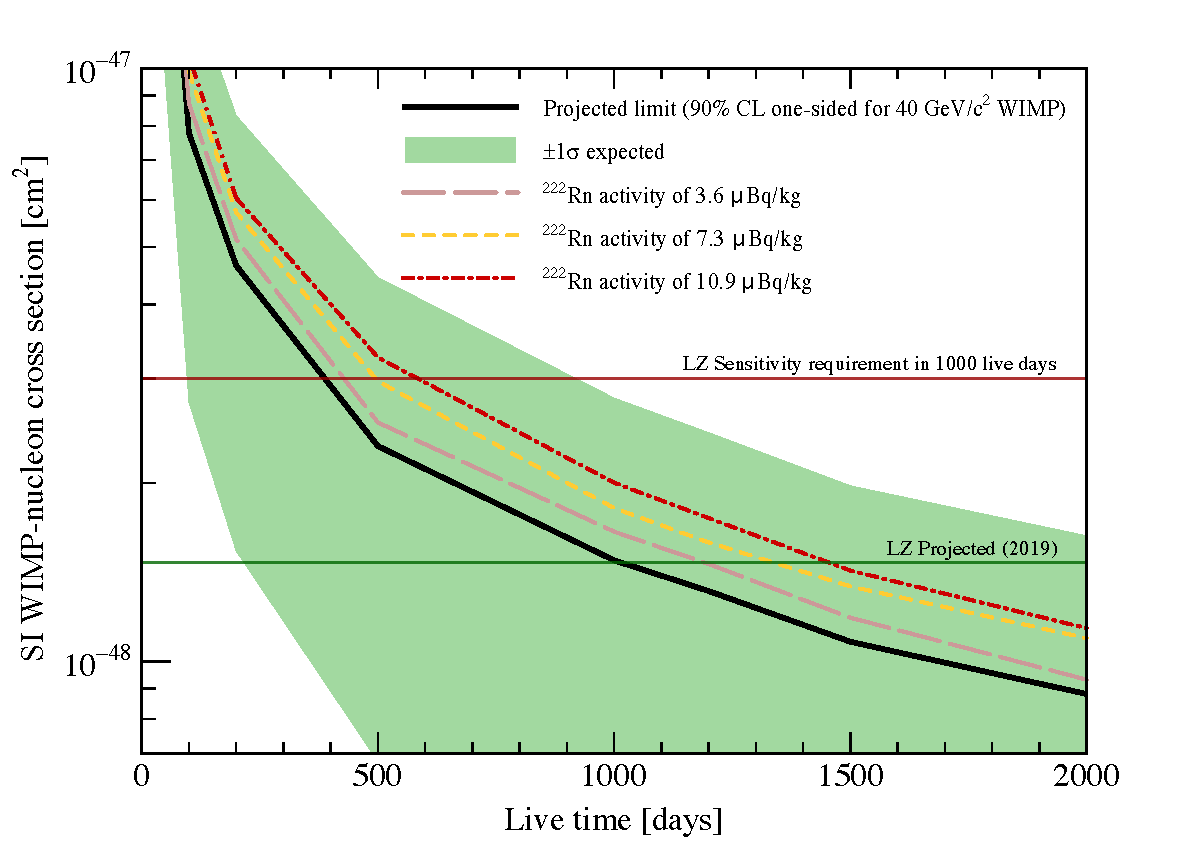
\includegraphics[scale=0.8]{Chapter_5/Figures/sensitivity_studies/sensitivity_vs_time_radon.pdf}
    \caption[Projected SI sensitivity in 5.6 tonnes of fiducial volume as a function of live days of data taking, showing the evolution of the median 90\% CL evolution for a range of \RnTTT{} activities for a WIMP mass of 40 GeV/c\squared{} WIMP.]%
    {Projected SI sensitivity in 5.6 tonnes of fiducial volume as a function of live days of data taking, showing the evolution of the median 90\% CL evolution for a range of \RnTTT{} activities for a WIMP mass of 40 GeV/c\squared{} WIMP. The baseline projected scenario with \RnTTT{} activity of 1.81 \micro{}Bq/kg is given as the solid black line, along with the $1\sigma$ band (green). The median sensitivity evolution for radon activities increase by factors of $x2$, $x4$, $x6$ are displayed in dashed coloured lines. The LZ sensitivity requirement and the baseline sensitivity is overlaid with horizontal red and green lines, respectively.}
    \label{fig:radon_vs_time}
\end{figure}
%

The SI-WIMP sensitivity against live days of data taking is shown in figure (\ref{fig:radon_vs_time}) for a multitude of radon activities. The solid black line in figure (\ref{fig:radon_vs_time}) shows the time evolution of the baseline scenario for the SI-WIMP sensitivity assuming a \RnTTT{} activity of 1.81 \micro{}Bq/kg across 0--2000 live days, overlaid with the $1\sigma$ band (solid green) of the median 90\% CL. Furthermore, the median 90\% CL sensitivity evolution of $x2$, $x4$, $x6$ radon activity factors in comparison to the baseline scenario is given as the dashed coloured lines, as indicated on the plot. As observed from the plot, doubling the \RnTTT{} activity to 3.6 \micro{}Bq/kg results in an extra $\sim48$ days above 1000 live days to regain the sensitivity loss in comparison to baseline projection. At a much larger radon activity---6 times the baseline projection, the impact becomes more substantial, where the baseline sensitivity is reached with an extra $\sim325$ live days.

In conclusion, the sensitivity studies detailed above on elevated radon levels within the active LXe volume of LZ indicate that the sensitivity and discovery potential to the SI-WIMP is not substantially impacted by even the worst case scenario arising from screening efforts. Despite the gradual increase in both sensitivity and discovery potential, a \RnTTT{} activity of 60.8 mBq results in a median sensitivity that remains below the LZ requirement \cite{lz_tdr, akerib2018projected}. Although the result is somewhat surprising, the \RnTTT{} background does indeed fall into the ER band, and ER-NR discrimination combined with the PLR analysis minimises the impact of such elevated radon levels. This is better understood when considering that although a shift in the \RnTTT{} normalisation increase the ER band population, it is the lower tail of the ER band distribution that leaks into the NR band. As can be seen from figures (\ref{fig:lz_1000_day_run} \& \ref{fig:lz_background_pdfs}), the denser regions of the ER and NR distributions remain fairly separated. In a conventional cut-and-count analysis, the leaked events are evenly distributed in the signal region, whereas in a PLR analysis, their relative positions in the $S1\mhyphen{}S2$ space is conserved, hence a large amount of the signal space remains undisturbed by larger ER backgrounds, resulting in a gradual loss in sensitivity and discovery potential. Although it appears that elevated levels of radon is not a large issue for the WIMP search, the impact of radon on signal models that are expected in the ER band will be much larger.

\clearpage

%%------------------------------$$
\section{Impact of Krypton on Sensitivity and Discovery Potential}
\label{sec:krypton_impact}
%%------------------------------$$

During the construction of the LZ detector, a parallel effort in purifying the sourced xenon from its radioactive contaminants was in place to remove the \KrEF{} by using a custom-made gas chromatography system. The removal of krypton is a time consuming process and reaching the ambitious requirement of 0.015 ppt of \KrEF{} set by the LZ TDR \cite{lz_tdr} in line with the construction of the detector and the incorporation of the xenon into the circulation system was in question. To determine whether the experiment can save time on krypton removal and deliver the xenon in time, a similar statistical study to that of radon for elevated \KrEF{} activities was conducted. 

The sensitivity and discovery potential to a 40 GeV/c\squared{} was examined over a range of \KrEF{} activities from 0.015--1.0 ppt. To incorporate the impact of elevated radon activity into this study, the \KrEF{} scenarios were examined under the nominal radon projection of 1.81 \micro{}Bq/kg and 3.62 \micro{}Bq/kg of xenon---twice the nominal rate. The expected number of \KrEF{} events showing up in the signal region of interest, derived from the cut-and-out analysis explained in section (\ref{secsec:background_table}) and given in table (\ref{tab:lz_background_count}), is 24.5 ER events in a 1000 live day run within the 5.6 tonne fiducial volume. As the krypton is expected to be uniformly dispersed within the LXe, the study was conducted by using the \textsc{LZStats} framework and altering the normalisation of the \KrEF{} distribution in the background model, $\mu_{^{85}Kr}$, for two \RnTTT{} scenarios. The median 90\% CL sensitivity and the $3\sigma$ discovery potential of varied \KrEF{} activities for both the nominal and twice the nominal projected radon levels are shown in figure (\ref{fig:krypton_sensitivity_discovery}). The irregularity observed in (\ref{fig:krypton_sensitivity_discovery}) is as a result of the lower statistics ($\sim10$k pseudo-experiments per hypothesis) used in assessing the impact of krypton.

As can be seen in figure (\ref{fig:lz_background_pdfs}), the \KrEF{} distribution is very similar to that of \RnTTT{}; with both residing in the ER band of the $S1\mhyphen{}S2$, hence the implication of an increased \KrEF{} to the SI-WIMP sensitivity is expected to be similar to that of radon. The objective key performance parameter (KPP) of 0.015 ppt and the threshold KKP of 0.3 ppt of \KrEF{} activity as defined by the LZ project is shown in dashed green and red lines in figure (\ref{fig:krypton_sensitivity_discovery}), respectively. For both scenarios of \RnTTT{}, the elevated levels of \KrEF{} activity results in a gradual increase in sensitivity and discovery potential; where the LZ sensitivity requirement is still achievable under the KPP threshold of 0.3 ppt of radon. The LZ sensitivity requirement remains to be achievable even at a much larger elevation of 1.0 ppt of \KrEF{} and twice the nominal radon projection. Although the SI-WIMP search is not drastically impacted by elevated levels of \KrEF{}, the overall goal of the experiment is to keep \KrEF{} concentrations well below the KPP threshold of 0.3 ppt, so to reduce the impact of \KrEF{} on ER physics searches.

%
\begin{figure}[h!]
    \centering
    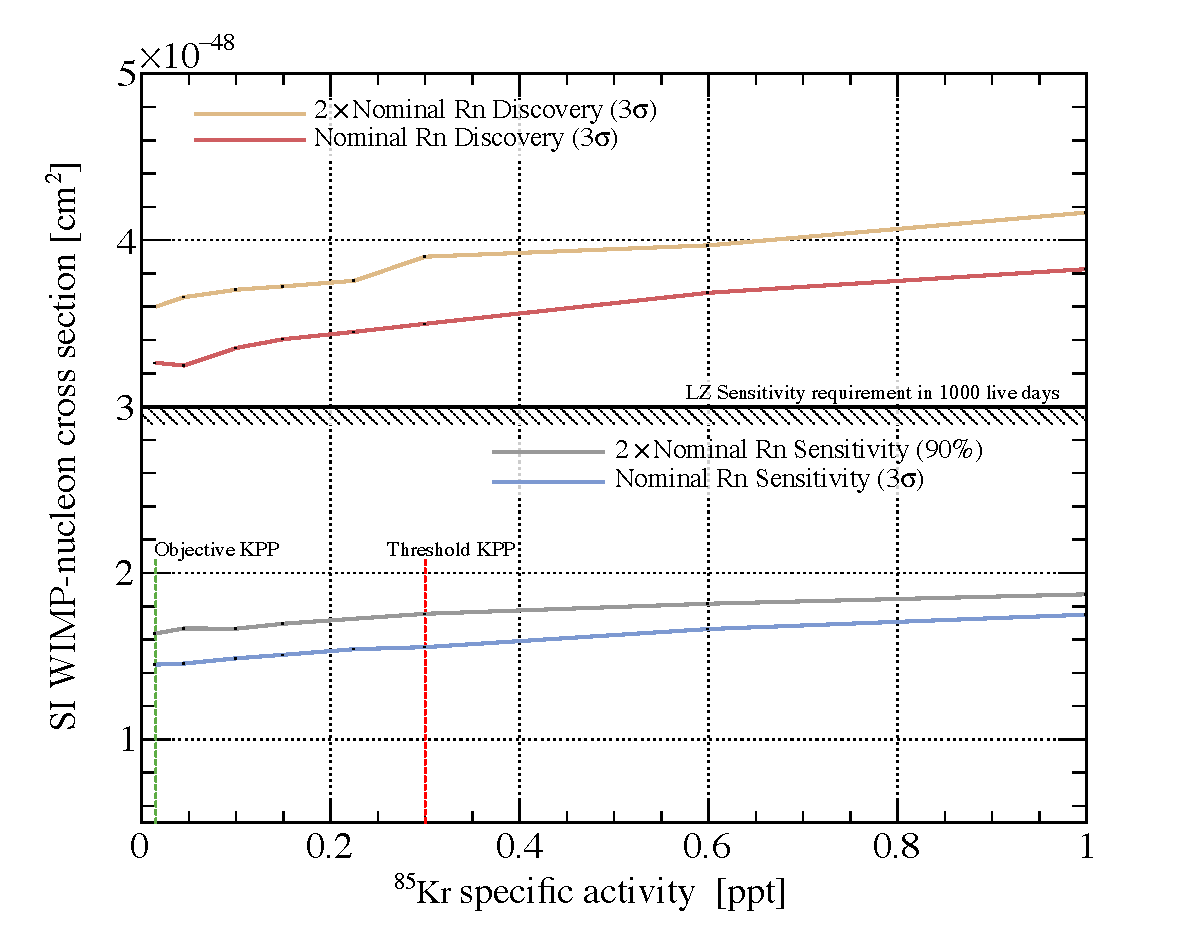
\includegraphics[scale=0.8]{Chapter_5/Figures/sensitivity_studies/lz_krypton_vs_sensitivity.pdf}
    \caption[Projected SI sensitivity and discovery potential for a 1000 live-days run in 5.6 tonnes of fiducial volume as a function of \KrEF{} as activity as observed in the fiducial volume for a WIMP mass of 40 GeV/c\squared{} WIMP.]%
    {Projected SI sensitivity and discovery potential for a 1000 live-days run in 5.6 tonnes of fiducial volume as a function of \KrEF{} as activity as observed in the fiducial volume for a WIMP mass of 40 GeV/c\squared{} WIMP. The median 90\% CL sensitivity and $3\sigma$ discovery potentials of \KrEF{} ranging from 0.015--1.0 ppt concentration are shown for two \RnTTT{} specific activities of 1.81 \micro{}Bk/kg and 3.62 \micro{}Bq/kg. The lower two curves show the variation in sensitivity, whereas the above two curves show the variation in discovery potential.}
    \label{fig:krypton_sensitivity_discovery}
\end{figure}
%

%%------------------------------$$
\section{Impact of veto Detectors on Sensitivity}
\label{sec:lz_veto_sensitivity}
%%------------------------------$$

SHALL I?

%%------------------------------$$
\section{Projected WIMP Sensitivity and Discovery Potential}
\label{sec:lz_sensitivity}
%%------------------------------$$

The projected LZ sensitivity and discovery potential to the SI WIMP-nucleon cross section at a 90\% CL is shown in figures (\ref{fig:projected_lz_sensitivity} \& \ref{fig:projected_lz_discovery}). The statistical studies are conducted over a wide range of WIMP masses varying from 5--2000 GeV/c\squared{}. Each mass is taken as an independent signal model in constructing the null and the alternative hypotheses, were a set of pseudo-experiments are generated for 20 test values of the POI ($\mu_{s}$), equally spaced between 0 to 30. In the limit setting scenario (above), for each mass, the test statistic distributions are used to determine the \textit{p}-values of the median, $1\sigma$ and the $2\sigma$ bands at the 90\% CL. In the case of discovery potential (below), the $3\sigma$ and $5\sigma$ potentials are determined, showing the region of parameter space above which the LZ experiment would have the ability to exclude the background-only hypothesis at the indicated significance.

The best sensitivity on the SI WIMP-nucleon cross section is expected for 40 GeV/c\squared{} WIMPs with a sensitivity of $1.43 \times 10^{-48} \; \MathText{cm}^2$, achieving a limit that is more than an order of magnitude lower than the limits set by recent LXe experiments \cite{lux_full, xenon_1t, pandax_limit}. As shown in figure (\ref{fig:projected_lz_sensitivity}), the projected median sensitivity, given as the solid black line, is expected to probe a significant fraction of the parameter space above the irreducible coherent neutrino scattering background, dubbed as the \textit{neutrino floor}, indicated as the shaded orange region. At a region closer to the neutrino floor, the NR signal region of WIMPs across all masses are saturated with nuclear recoils from coherent elastic neutrino-nucleus scattering, significantly reducing the sensitivity improvements from experimental scaling. At lower WIMP masses ($\leqslant10$ GeV/c\squared{}), the presence of neutrino backgrounds from \BE{} and \textit{hep} is already limiting the sensitivity gains made my larger scale experiments. However, although the coherent elastic neutrino-nucleus scattering is becoming significantly more constraining for WIMP searches in LXe, studying CE$\nu$NS with LXe detectors can pave the way for a better understanding of their flux and hence improve future WIMP searches with more precise modeling of these backgrounds. For LZ, the low energy event rates for background and signal modeling will ultimately depend on the low energy nuclear recoil efficiency of the experiment, which is currently capped at 1.1 keV due to the limitations of experimental data below this energy.  

Furthermore, the $3s\sigma$ and $5\sigma$ discovery potential for the SI WIMP-nucleon scattering is shown as a function of WIMP mass and compared with the 90\% CL sensitivity in figure (\ref{fig:projected_lz_discovery}). In conducting these studies, the median of the alternative distribution is taken as teh value of the observed test statistic and hence, these projections represent the outcome of the median experiment over repeated realisations. At 40 GeV/c\squared{}, the median $3\sigma$ and $5\sigma$ significance is projected to occur at $3.4 \times 10^{-48} \; \MathText{cm}^2$ and $6.5 \times 10^{-48} \; \MathText{cm}^2$. Across all tested WIMP masses, the projected $3\sigma$ and $5\sigma$ significance is below the 90\% CL limits from recent experiments, leaving a significant region of the parameter space open for the discovery of a SI WIMP signal with the LZ experiment.

%
\begin{figure}[h!]
    \centering
    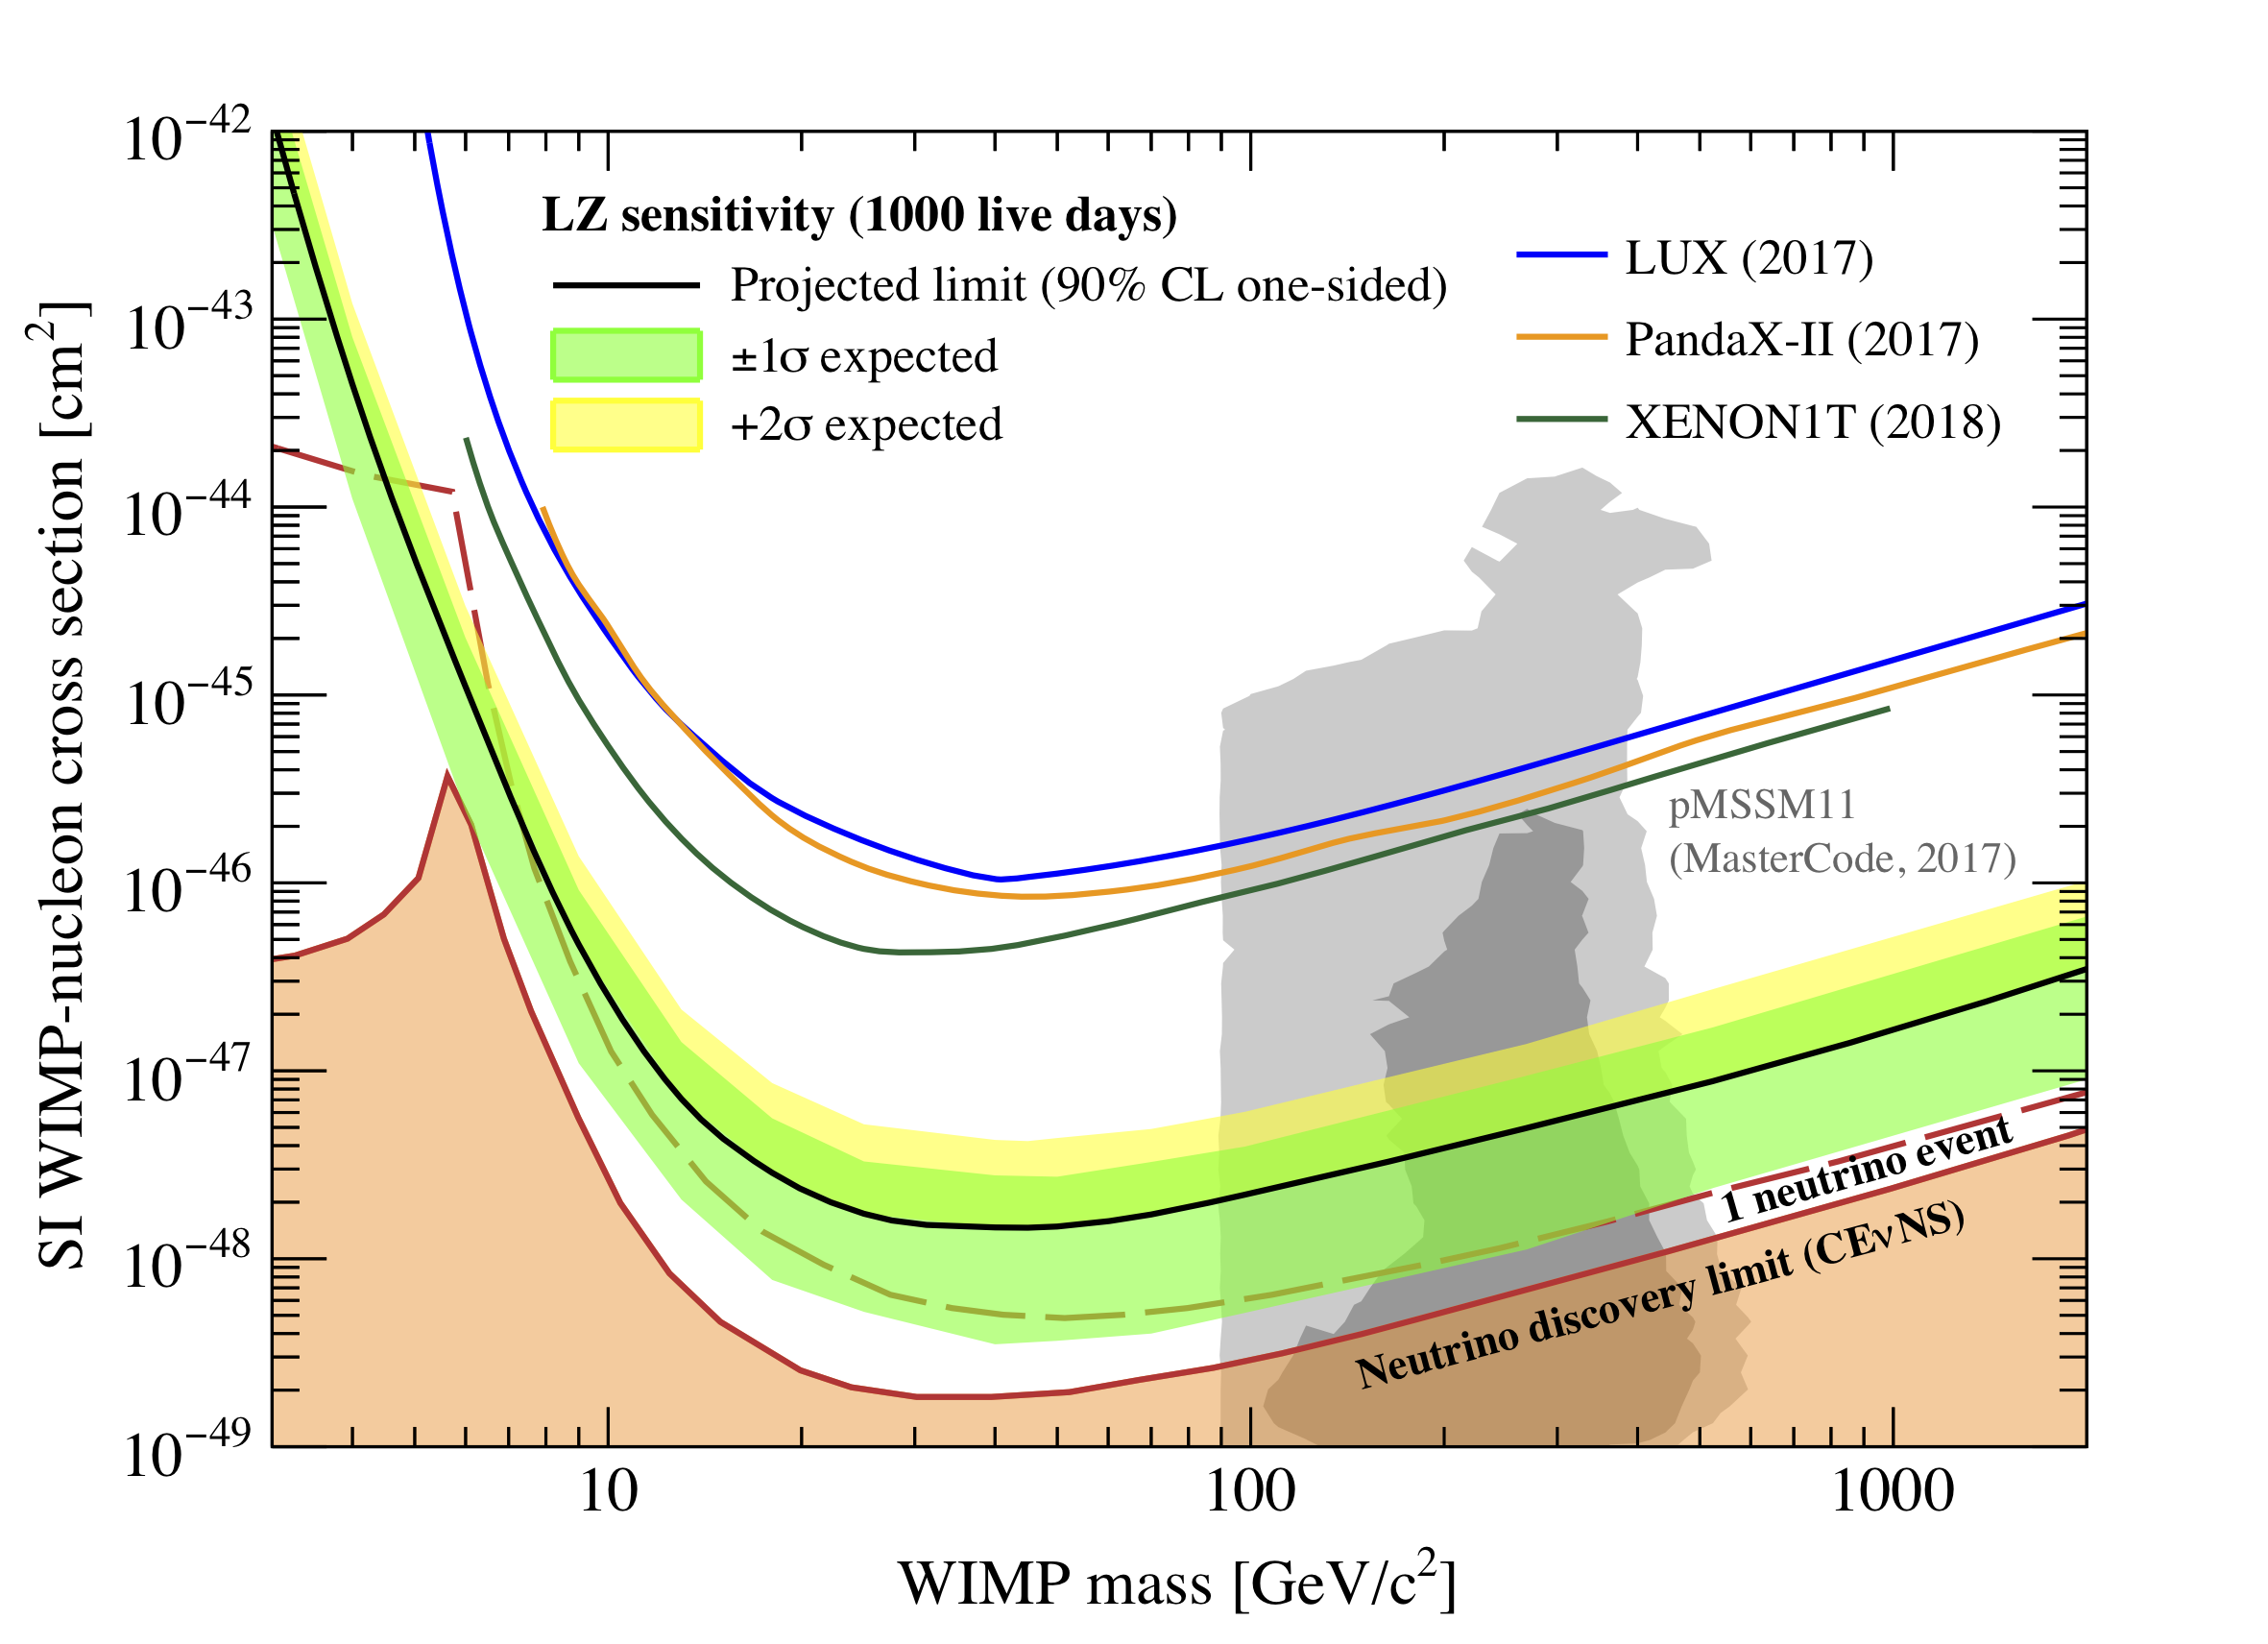
\includegraphics[scale=0.8]{Chapter_5/Figures/sensitivity_studies/lz_projection_1000_day.png}
    \caption[LZ projected sensitivity to the SI WIMP-nucleon elastic scattering for 1000 live days and a 5.6 tonne fiducial volume in WIMP search region of interest.]%
    {LZ projected sensitivity (above) and discovery potential (below) to the SI WIMP-nucleon elastic scattering for 1000 live days and a 5.6 tonne fiducial volume in WIMP search region of interest. The best median 90\% CL sensitivity of $1.43 \times 10^{-48} \; \MathText{cm}^2$ is achieved at a WIMP mass of 40 GeV/c\squared{} (solid black line). The $-2\sigma$ expected region is omitted based on the expectation that the limit will be power constrained \cite{Cowan:2011an}. Recent results achieved by other LXe experiments are also shown for comparison \cite{lux_full, xenon_1t, pandax_limit}. The lower shaded region and dashed line indicate the emergence of backgrounds from coherent scattering of neutrinos \cite{neutrino_floor} and the gray contoured regions show the favored regions from recent pMSSM11 model scans \cite{pMSSM11}.}
    \label{fig:projected_lz_sensitivity}
\end{figure}
%

%
\begin{figure}[H!]
    \centering
    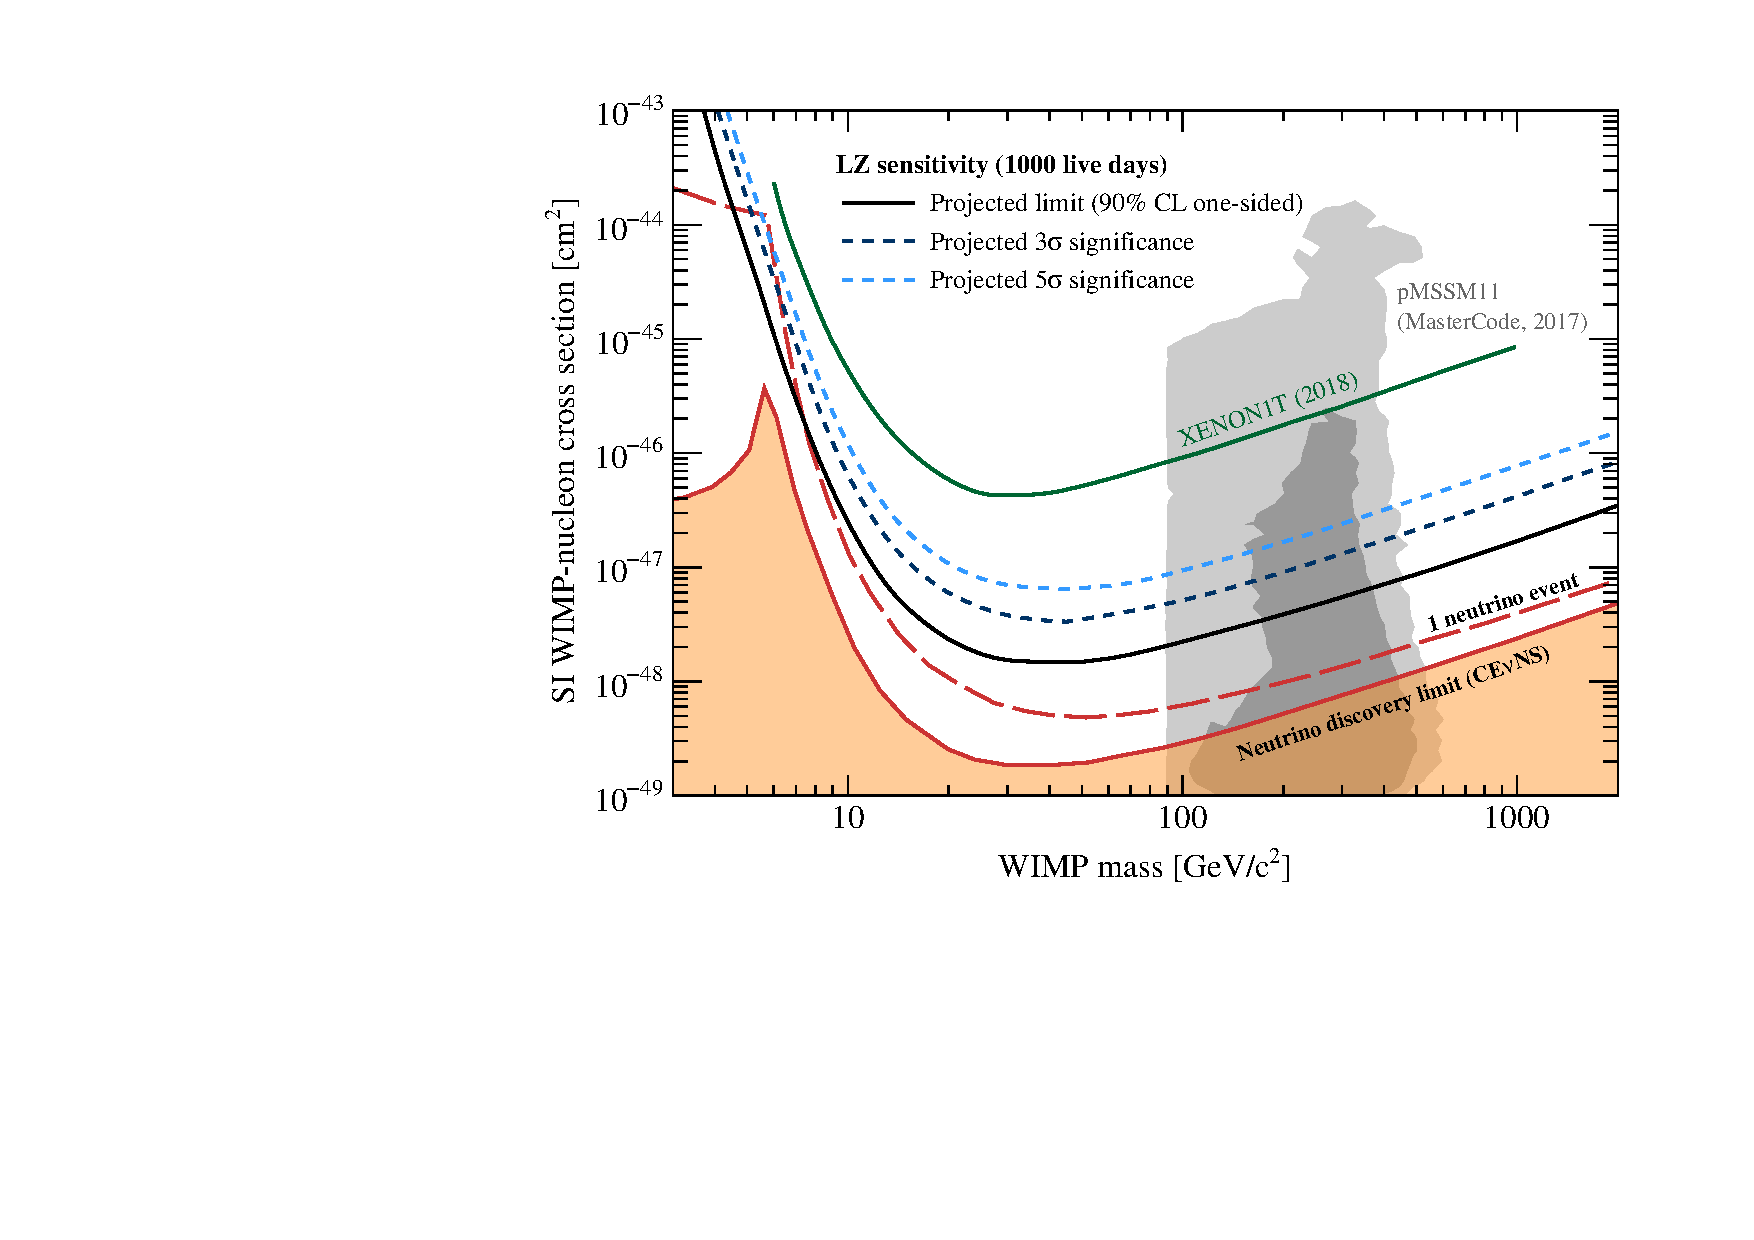
\includegraphics[scale=0.8]{Chapter_5/Figures/sensitivity_studies/lz_discovery_1000_day.pdf}
    \caption[LZ projected discovery potential to the SI WIMP-nucleon elastic scattering for 1000 live days and a 5.6 tonne fiducial volume in WIMP search region of interest.]%
    {LZ projected discovery potential (below) to the SI WIMP-nucleon elastic scattering for 1000 live days and a 5.6 tonne fiducial volume in WIMP search region of interest. The best 3(5)$\sigma$ significance is achieved at $3.4(6.5) \times 10^{-48} \; \MathText{cm}^{2}$ for 40 GeV/c\squared{} WIMPs. The current best limit XENON1T is shown for comparison \cite{xenon_1t}. Figure adapted from \cite{akerib2018projected}.}
    \label{fig:projected_lz_discovery}
\end{figure}
%


